\documentclass[twoside]{book}

% Packages required by doxygen
\usepackage{fixltx2e}
\usepackage{calc}
\usepackage{doxygen}
\usepackage[export]{adjustbox} % also loads graphicx
\usepackage{graphicx}
\usepackage[utf8]{inputenc}
\usepackage{makeidx}
\usepackage{multicol}
\usepackage{multirow}
\PassOptionsToPackage{warn}{textcomp}
\usepackage{textcomp}
\usepackage[nointegrals]{wasysym}
\usepackage[table]{xcolor}

% Font selection
\usepackage[T1]{fontenc}
\usepackage[scaled=.90]{helvet}
\usepackage{courier}
\usepackage{amssymb}
\usepackage{sectsty}
\renewcommand{\familydefault}{\sfdefault}
\allsectionsfont{%
  \fontseries{bc}\selectfont%
  \color{darkgray}%
}
\renewcommand{\DoxyLabelFont}{%
  \fontseries{bc}\selectfont%
  \color{darkgray}%
}
\newcommand{\+}{\discretionary{\mbox{\scriptsize$\hookleftarrow$}}{}{}}

% Page & text layout
\usepackage{geometry}
\geometry{%
  a4paper,%
  top=2.5cm,%
  bottom=2.5cm,%
  left=2.5cm,%
  right=2.5cm%
}
\tolerance=750
\hfuzz=15pt
\hbadness=750
\setlength{\emergencystretch}{15pt}
\setlength{\parindent}{0cm}
\setlength{\parskip}{3ex plus 2ex minus 2ex}
\makeatletter
\renewcommand{\paragraph}{%
  \@startsection{paragraph}{4}{0ex}{-1.0ex}{1.0ex}{%
    \normalfont\normalsize\bfseries\SS@parafont%
  }%
}
\renewcommand{\subparagraph}{%
  \@startsection{subparagraph}{5}{0ex}{-1.0ex}{1.0ex}{%
    \normalfont\normalsize\bfseries\SS@subparafont%
  }%
}
\makeatother

% Headers & footers
\usepackage{fancyhdr}
\pagestyle{fancyplain}
\fancyhead[LE]{\fancyplain{}{\bfseries\thepage}}
\fancyhead[CE]{\fancyplain{}{}}
\fancyhead[RE]{\fancyplain{}{\bfseries\leftmark}}
\fancyhead[LO]{\fancyplain{}{\bfseries\rightmark}}
\fancyhead[CO]{\fancyplain{}{}}
\fancyhead[RO]{\fancyplain{}{\bfseries\thepage}}
\fancyfoot[LE]{\fancyplain{}{}}
\fancyfoot[CE]{\fancyplain{}{}}
\fancyfoot[RE]{\fancyplain{}{\bfseries\scriptsize Generated by Doxygen }}
\fancyfoot[LO]{\fancyplain{}{\bfseries\scriptsize Generated by Doxygen }}
\fancyfoot[CO]{\fancyplain{}{}}
\fancyfoot[RO]{\fancyplain{}{}}
\renewcommand{\footrulewidth}{0.4pt}
\renewcommand{\chaptermark}[1]{%
  \markboth{#1}{}%
}
\renewcommand{\sectionmark}[1]{%
  \markright{\thesection\ #1}%
}

% Indices & bibliography
\usepackage{natbib}
\usepackage[titles]{tocloft}
\setcounter{tocdepth}{3}
\setcounter{secnumdepth}{5}
\makeindex

% Hyperlinks (required, but should be loaded last)
\usepackage{ifpdf}
\ifpdf
  \usepackage[pdftex,pagebackref=true]{hyperref}
\else
  \usepackage[ps2pdf,pagebackref=true]{hyperref}
\fi
\hypersetup{%
  colorlinks=true,%
  linkcolor=blue,%
  citecolor=blue,%
  unicode%
}

% Custom commands
\newcommand{\clearemptydoublepage}{%
  \newpage{\pagestyle{empty}\cleardoublepage}%
}

\usepackage{caption}
\captionsetup{labelsep=space,justification=centering,font={bf},singlelinecheck=off,skip=4pt,position=top}

%===== C O N T E N T S =====

\begin{document}

% Titlepage & ToC
\hypersetup{pageanchor=false,
             bookmarksnumbered=true,
             pdfencoding=unicode
            }
\pagenumbering{alph}
\begin{titlepage}
\vspace*{7cm}
\begin{center}%
{\Large Sumfactorization }\\
\vspace*{1cm}
{\large Generated by Doxygen 1.8.14}\\
\end{center}
\end{titlepage}
\clearemptydoublepage
\pagenumbering{roman}
\tableofcontents
\clearemptydoublepage
\pagenumbering{arabic}
\hypersetup{pageanchor=true}

%--- Begin generated contents ---
\chapter{Namespace Index}
\section{Namespace List}
Here is a list of all namespaces with brief descriptions\+:\begin{DoxyCompactList}
\item\contentsline{section}{\hyperlink{namespacemath}{math} }{\pageref{namespacemath}}{}
\item\contentsline{section}{\hyperlink{namespacemath_1_1detail}{math\+::detail} }{\pageref{namespacemath_1_1detail}}{}
\end{DoxyCompactList}

\chapter{Hierarchical Index}
\section{Class Hierarchy}
This inheritance list is sorted roughly, but not completely, alphabetically\+:\begin{DoxyCompactList}
\item \contentsline{section}{constexpr\+\_\+array$<$ T, N $>$}{\pageref{classconstexpr__array}}{}
\item \contentsline{section}{constexpr\+\_\+array$<$ q\+\_\+order, order+1 $>$}{\pageref{classconstexpr__array}}{}
\item \contentsline{section}{constexpr\+\_\+array$<$ y\+\_\+type, order+1 $>$}{\pageref{classconstexpr__array}}{}
\item \contentsline{section}{math\+:\+:detail\+:\+:gen\+\_\+seq$<$ N, Is $>$}{\pageref{structmath_1_1detail_1_1gen__seq}}{}
\item \contentsline{section}{Integrate$<$ order, y\+\_\+type, Polynomial, Quadrature $>$}{\pageref{class_integrate}}{}
\item \contentsline{section}{Polynomial$<$ order, y\+\_\+type, Quadrature $>$}{\pageref{class_polynomial}}{}
\item \contentsline{section}{Polynomial$<$ order, y\+\_\+type $>$}{\pageref{class_polynomial}}{}
\item \contentsline{section}{Quadrature$<$ y\+\_\+type, order $>$}{\pageref{class_quadrature}}{}
\item \contentsline{section}{Quadrature$<$ q\+\_\+order, y\+\_\+type $>$}{\pageref{class_quadrature}}{}
\item \contentsline{section}{math\+:\+:detail\+:\+:seq$<$ Is $>$}{\pageref{structmath_1_1detail_1_1seq}}{}
\item \contentsline{section}{math\+:\+:detail\+:\+:seq$<$ Is... $>$}{\pageref{structmath_1_1detail_1_1seq}}{}
\begin{DoxyCompactList}
\item \contentsline{section}{math\+:\+:detail\+:\+:gen\+\_\+seq$<$ 0, Is... $>$}{\pageref{structmath_1_1detail_1_1gen__seq_3_010_00_01_is_8_8_8_01_4}}{}
\end{DoxyCompactList}
\item \contentsline{section}{math\+:\+:detail\+:\+:sin\+\_\+coeffs$<$ T, N $>$}{\pageref{structmath_1_1detail_1_1sin__coeffs}}{}
\item \contentsline{section}{V\+M\+U\+LT$<$ order, q\+\_\+order, c, y\+\_\+type, Polynomial, Quadrature $>$}{\pageref{class_v_m_u_l_t}}{}
\end{DoxyCompactList}

\chapter{Class Index}
\section{Class List}
Here are the classes, structs, unions and interfaces with brief descriptions\+:\begin{DoxyCompactList}
\item\contentsline{section}{\hyperlink{classconstexpr__array}{constexpr\+\_\+array$<$ T, N $>$} }{\pageref{classconstexpr__array}}{}
\item\contentsline{section}{\hyperlink{structmath_1_1detail_1_1gen__seq}{math\+::detail\+::gen\+\_\+seq$<$ N, Is $>$} }{\pageref{structmath_1_1detail_1_1gen__seq}}{}
\item\contentsline{section}{\hyperlink{structmath_1_1detail_1_1gen__seq_3_010_00_01_is_8_8_8_01_4}{math\+::detail\+::gen\+\_\+seq$<$ 0, Is... $>$} }{\pageref{structmath_1_1detail_1_1gen__seq_3_010_00_01_is_8_8_8_01_4}}{}
\item\contentsline{section}{\hyperlink{class_integrate}{Integrate$<$ order, y\+\_\+type, Polynomial, Quadrature $>$} }{\pageref{class_integrate}}{}
\item\contentsline{section}{\hyperlink{class_polynomial}{Polynomial$<$ order, y\+\_\+type, Quadrature $>$} }{\pageref{class_polynomial}}{}
\item\contentsline{section}{\hyperlink{class_quadrature}{Quadrature$<$ y\+\_\+type, order $>$} }{\pageref{class_quadrature}}{}
\item\contentsline{section}{\hyperlink{structmath_1_1detail_1_1seq}{math\+::detail\+::seq$<$ Is $>$} }{\pageref{structmath_1_1detail_1_1seq}}{}
\item\contentsline{section}{\hyperlink{structmath_1_1detail_1_1sin__coeffs}{math\+::detail\+::sin\+\_\+coeffs$<$ T, N $>$} }{\pageref{structmath_1_1detail_1_1sin__coeffs}}{}
\item\contentsline{section}{\hyperlink{class_v_m_u_l_t}{V\+M\+U\+L\+T$<$ order, q\+\_\+order, c, y\+\_\+type, Polynomial, Quadrature $>$} }{\pageref{class_v_m_u_l_t}}{}
\end{DoxyCompactList}

\chapter{File Index}
\section{File List}
Here is a list of all files with brief descriptions\+:\begin{DoxyCompactList}
\item\contentsline{section}{build/\+C\+Make\+Files/\hyperlink{feature__tests_8c}{feature\+\_\+tests.\+c} }{\pageref{feature__tests_8c}}{}
\item\contentsline{section}{build/\+C\+Make\+Files/\hyperlink{feature__tests_8cxx}{feature\+\_\+tests.\+cxx} }{\pageref{feature__tests_8cxx}}{}
\item\contentsline{section}{build/\+C\+Make\+Files/3.\+7.\+1/\+Compiler\+Id\+C/\hyperlink{_c_make_c_compiler_id_8c}{C\+Make\+C\+Compiler\+Id.\+c} }{\pageref{_c_make_c_compiler_id_8c}}{}
\item\contentsline{section}{build/\+C\+Make\+Files/3.\+7.\+1/\+Compiler\+Id\+C\+X\+X/\hyperlink{_c_make_c_x_x_compiler_id_8cpp}{C\+Make\+C\+X\+X\+Compiler\+Id.\+cpp} }{\pageref{_c_make_c_x_x_compiler_id_8cpp}}{}
\item\contentsline{section}{include/\hyperlink{constexpr__array_8h}{constexpr\+\_\+array.\+h} }{\pageref{constexpr__array_8h}}{}
\item\contentsline{section}{include/\hyperlink{integrate_8h}{integrate.\+h} }{\pageref{integrate_8h}}{}
\item\contentsline{section}{include/\hyperlink{la__operations_8h}{la\+\_\+operations.\+h} }{\pageref{la__operations_8h}}{}
\item\contentsline{section}{include/\hyperlink{math__constexpr_8h}{math\+\_\+constexpr.\+h} }{\pageref{math__constexpr_8h}}{}
\item\contentsline{section}{include/\hyperlink{polynomial_8h}{polynomial.\+h} }{\pageref{polynomial_8h}}{}
\item\contentsline{section}{include/\hyperlink{quadrature_8h}{quadrature.\+h} }{\pageref{quadrature_8h}}{}
\item\contentsline{section}{include/\hyperlink{quadrature__constexpr_8h}{quadrature\+\_\+constexpr.\+h} }{\pageref{quadrature__constexpr_8h}}{}
\item\contentsline{section}{include/\hyperlink{vmult_8h}{vmult.\+h} }{\pageref{vmult_8h}}{}
\item\contentsline{section}{tests/\hyperlink{integrate_8cc}{integrate.\+cc} }{\pageref{integrate_8cc}}{}
\item\contentsline{section}{tests/\hyperlink{polynomial_8cc}{polynomial.\+cc} }{\pageref{polynomial_8cc}}{}
\item\contentsline{section}{tests/\hyperlink{quadrature_8cc}{quadrature.\+cc} }{\pageref{quadrature_8cc}}{}
\end{DoxyCompactList}

\chapter{Namespace Documentation}
\hypertarget{namespacemath}{}\section{math Namespace Reference}
\label{namespacemath}\index{math@{math}}
\subsection*{Namespaces}
\begin{DoxyCompactItemize}
\item 
 \hyperlink{namespacemath_1_1detail}{detail}
\end{DoxyCompactItemize}
\subsection*{Functions}
\begin{DoxyCompactItemize}
\item 
{\footnotesize template$<$typename y\+\_\+type $>$ }\\constexpr y\+\_\+type \hyperlink{namespacemath_a4ed3724aa337c68adee88563238c6845}{fabs} (y\+\_\+type val)
\item 
{\footnotesize template$<$class T , class dcy  = std\+::decay\+\_\+t$<$\+T$>$$>$ }\\constexpr std\+::enable\+\_\+if\+\_\+t$<$ std\+::is\+\_\+floating\+\_\+point$<$ T $>$\+::value, dcy $>$ \hyperlink{namespacemath_ad1f27e28f460fb7a1393d9c0518c2e53}{inverse} (T value)
\item 
{\footnotesize template$<$class T $>$ }\\constexpr std\+::decay\+\_\+t$<$ T $>$ \hyperlink{namespacemath_a9fed6bdc392a6c857d3d1a93f735e243}{sign} (T value)
\item 
{\footnotesize template$<$typename T $>$ }\\constexpr std\+::decay\+\_\+t$<$ T $>$ \hyperlink{namespacemath_a49650a9f506dd5208d963d74ab9b9370}{abs} (T value)
\item 
{\footnotesize template$<$class T $>$ }\\constexpr std\+::decay\+\_\+t$<$ T $>$ \hyperlink{namespacemath_a096802f59879957bb79b461ee9a0ddf9}{power} (T const \&base, std\+::size\+\_\+t const \&pow)
\item 
constexpr std\+::intmax\+\_\+t \hyperlink{namespacemath_a7606ea45ee84c24d1a0e661bec3879f1}{factorial} (std\+::intmax\+\_\+t const \&n)
\item 
{\footnotesize template$<$class T , std\+::size\+\_\+t N = max\+\_\+factorial, class dcy  = std\+::decay\+\_\+t$<$\+T$>$$>$ }\\constexpr std\+::enable\+\_\+if\+\_\+t$<$ std\+::is\+\_\+floating\+\_\+point$<$ dcy $>$\+::value, dcy $>$ \hyperlink{namespacemath_a82b6cd9ca916160f03a5d1450eb7a009}{sin} (T x) noexcept
\end{DoxyCompactItemize}


\subsection{Function Documentation}
\mbox{\Hypertarget{namespacemath_a49650a9f506dd5208d963d74ab9b9370}\label{namespacemath_a49650a9f506dd5208d963d74ab9b9370}} 
\index{math@{math}!abs@{abs}}
\index{abs@{abs}!math@{math}}
\subsubsection{\texorpdfstring{abs()}{abs()}}
{\footnotesize\ttfamily template$<$typename T $>$ \\
constexpr std\+::decay\+\_\+t$<$T$>$ math\+::abs (\begin{DoxyParamCaption}\item[{T}]{value }\end{DoxyParamCaption})\hspace{0.3cm}{\ttfamily [inline]}}

\mbox{\Hypertarget{namespacemath_a4ed3724aa337c68adee88563238c6845}\label{namespacemath_a4ed3724aa337c68adee88563238c6845}} 
\index{math@{math}!fabs@{fabs}}
\index{fabs@{fabs}!math@{math}}
\subsubsection{\texorpdfstring{fabs()}{fabs()}}
{\footnotesize\ttfamily template$<$typename y\+\_\+type $>$ \\
constexpr y\+\_\+type math\+::fabs (\begin{DoxyParamCaption}\item[{y\+\_\+type}]{val }\end{DoxyParamCaption})}

\mbox{\Hypertarget{namespacemath_a7606ea45ee84c24d1a0e661bec3879f1}\label{namespacemath_a7606ea45ee84c24d1a0e661bec3879f1}} 
\index{math@{math}!factorial@{factorial}}
\index{factorial@{factorial}!math@{math}}
\subsubsection{\texorpdfstring{factorial()}{factorial()}}
{\footnotesize\ttfamily constexpr std\+::intmax\+\_\+t math\+::factorial (\begin{DoxyParamCaption}\item[{std\+::intmax\+\_\+t const \&}]{n }\end{DoxyParamCaption})}

\mbox{\Hypertarget{namespacemath_ad1f27e28f460fb7a1393d9c0518c2e53}\label{namespacemath_ad1f27e28f460fb7a1393d9c0518c2e53}} 
\index{math@{math}!inverse@{inverse}}
\index{inverse@{inverse}!math@{math}}
\subsubsection{\texorpdfstring{inverse()}{inverse()}}
{\footnotesize\ttfamily template$<$class T , class dcy  = std\+::decay\+\_\+t$<$\+T$>$$>$ \\
constexpr std\+::enable\+\_\+if\+\_\+t$<$std\+::is\+\_\+floating\+\_\+point$<$T$>$\+::value,dcy$>$ math\+::inverse (\begin{DoxyParamCaption}\item[{T}]{value }\end{DoxyParamCaption})\hspace{0.3cm}{\ttfamily [inline]}}

\mbox{\Hypertarget{namespacemath_a096802f59879957bb79b461ee9a0ddf9}\label{namespacemath_a096802f59879957bb79b461ee9a0ddf9}} 
\index{math@{math}!power@{power}}
\index{power@{power}!math@{math}}
\subsubsection{\texorpdfstring{power()}{power()}}
{\footnotesize\ttfamily template$<$class T $>$ \\
constexpr std\+::decay\+\_\+t$<$T$>$ math\+::power (\begin{DoxyParamCaption}\item[{T const \&}]{base,  }\item[{std\+::size\+\_\+t const \&}]{pow }\end{DoxyParamCaption})\hspace{0.3cm}{\ttfamily [inline]}}

\mbox{\Hypertarget{namespacemath_a9fed6bdc392a6c857d3d1a93f735e243}\label{namespacemath_a9fed6bdc392a6c857d3d1a93f735e243}} 
\index{math@{math}!sign@{sign}}
\index{sign@{sign}!math@{math}}
\subsubsection{\texorpdfstring{sign()}{sign()}}
{\footnotesize\ttfamily template$<$class T $>$ \\
constexpr std\+::decay\+\_\+t$<$T$>$ math\+::sign (\begin{DoxyParamCaption}\item[{T}]{value }\end{DoxyParamCaption})\hspace{0.3cm}{\ttfamily [inline]}}

\mbox{\Hypertarget{namespacemath_a82b6cd9ca916160f03a5d1450eb7a009}\label{namespacemath_a82b6cd9ca916160f03a5d1450eb7a009}} 
\index{math@{math}!sin@{sin}}
\index{sin@{sin}!math@{math}}
\subsubsection{\texorpdfstring{sin()}{sin()}}
{\footnotesize\ttfamily template$<$class T , std\+::size\+\_\+t N = max\+\_\+factorial, class dcy  = std\+::decay\+\_\+t$<$\+T$>$$>$ \\
constexpr std\+::enable\+\_\+if\+\_\+t$<$std\+::is\+\_\+floating\+\_\+point$<$dcy$>$\+::value,dcy$>$ math\+::sin (\begin{DoxyParamCaption}\item[{T}]{x }\end{DoxyParamCaption})\hspace{0.3cm}{\ttfamily [noexcept]}}


\hypertarget{namespacemath_1_1detail}{}\section{math\+:\+:detail Namespace Reference}
\label{namespacemath_1_1detail}\index{math\+::detail@{math\+::detail}}
\subsection*{Classes}
\begin{DoxyCompactItemize}
\item 
struct \hyperlink{structmath_1_1detail_1_1gen__seq}{gen\+\_\+seq}
\item 
struct \hyperlink{structmath_1_1detail_1_1gen__seq_3_010_00_01_is_8_8_8_01_4}{gen\+\_\+seq$<$ 0, Is... $>$}
\item 
struct \hyperlink{structmath_1_1detail_1_1seq}{seq}
\item 
struct \hyperlink{structmath_1_1detail_1_1sin__coeffs}{sin\+\_\+coeffs}
\end{DoxyCompactItemize}

\chapter{Class Documentation}
\hypertarget{classconstexpr__array}{}\section{constexpr\+\_\+array$<$ T, N $>$ Class Template Reference}
\label{classconstexpr__array}\index{constexpr\+\_\+array$<$ T, N $>$@{constexpr\+\_\+array$<$ T, N $>$}}


{\ttfamily \#include $<$constexpr\+\_\+array.\+h$>$}

\subsection*{Public Types}
\begin{DoxyCompactItemize}
\item 
using \hyperlink{classconstexpr__array_a649b2a387e5109c7750c536a3518ab3e}{iterator} = T $\ast$
\end{DoxyCompactItemize}
\subsection*{Public Member Functions}
\begin{DoxyCompactItemize}
\item 
constexpr size\+\_\+t \hyperlink{classconstexpr__array_ae6cbbf0ef54c3df192c861572e4a2d5d}{size} () const
\item 
constexpr T \& \hyperlink{classconstexpr__array_a361c0575453f2ae3a363dbd35cd94a8e}{operator\mbox{[}$\,$\mbox{]}} (size\+\_\+t n)
\item 
constexpr const T \& \hyperlink{classconstexpr__array_af4dbc25da16e0e08bedb1d37693eda34}{operator\mbox{[}$\,$\mbox{]}} (size\+\_\+t n) const
\item 
constexpr \hyperlink{classconstexpr__array_a649b2a387e5109c7750c536a3518ab3e}{iterator} \hyperlink{classconstexpr__array_a405f736c800b2cd4527d1b574a56e5af}{begin} ()
\item 
constexpr \hyperlink{classconstexpr__array_a649b2a387e5109c7750c536a3518ab3e}{iterator} \hyperlink{classconstexpr__array_ad3680b32e76738116dbb9c0efeca5bd4}{end} ()
\end{DoxyCompactItemize}


\subsection{Member Typedef Documentation}
\mbox{\Hypertarget{classconstexpr__array_a649b2a387e5109c7750c536a3518ab3e}\label{classconstexpr__array_a649b2a387e5109c7750c536a3518ab3e}} 
\index{constexpr\+\_\+array@{constexpr\+\_\+array}!iterator@{iterator}}
\index{iterator@{iterator}!constexpr\+\_\+array@{constexpr\+\_\+array}}
\subsubsection{\texorpdfstring{iterator}{iterator}}
{\footnotesize\ttfamily template$<$typename T, size\+\_\+t N$>$ \\
using \hyperlink{classconstexpr__array}{constexpr\+\_\+array}$<$ T, N $>$\+::\hyperlink{classconstexpr__array_a649b2a387e5109c7750c536a3518ab3e}{iterator} =  T$\ast$}



\subsection{Member Function Documentation}
\mbox{\Hypertarget{classconstexpr__array_a405f736c800b2cd4527d1b574a56e5af}\label{classconstexpr__array_a405f736c800b2cd4527d1b574a56e5af}} 
\index{constexpr\+\_\+array@{constexpr\+\_\+array}!begin@{begin}}
\index{begin@{begin}!constexpr\+\_\+array@{constexpr\+\_\+array}}
\subsubsection{\texorpdfstring{begin()}{begin()}}
{\footnotesize\ttfamily template$<$typename T, size\+\_\+t N$>$ \\
constexpr \hyperlink{classconstexpr__array_a649b2a387e5109c7750c536a3518ab3e}{iterator} \hyperlink{classconstexpr__array}{constexpr\+\_\+array}$<$ T, N $>$\+::begin (\begin{DoxyParamCaption}{ }\end{DoxyParamCaption})\hspace{0.3cm}{\ttfamily [inline]}}

\mbox{\Hypertarget{classconstexpr__array_ad3680b32e76738116dbb9c0efeca5bd4}\label{classconstexpr__array_ad3680b32e76738116dbb9c0efeca5bd4}} 
\index{constexpr\+\_\+array@{constexpr\+\_\+array}!end@{end}}
\index{end@{end}!constexpr\+\_\+array@{constexpr\+\_\+array}}
\subsubsection{\texorpdfstring{end()}{end()}}
{\footnotesize\ttfamily template$<$typename T, size\+\_\+t N$>$ \\
constexpr \hyperlink{classconstexpr__array_a649b2a387e5109c7750c536a3518ab3e}{iterator} \hyperlink{classconstexpr__array}{constexpr\+\_\+array}$<$ T, N $>$\+::end (\begin{DoxyParamCaption}{ }\end{DoxyParamCaption})\hspace{0.3cm}{\ttfamily [inline]}}

\mbox{\Hypertarget{classconstexpr__array_a361c0575453f2ae3a363dbd35cd94a8e}\label{classconstexpr__array_a361c0575453f2ae3a363dbd35cd94a8e}} 
\index{constexpr\+\_\+array@{constexpr\+\_\+array}!operator\mbox{[}\mbox{]}@{operator[]}}
\index{operator\mbox{[}\mbox{]}@{operator[]}!constexpr\+\_\+array@{constexpr\+\_\+array}}
\subsubsection{\texorpdfstring{operator[]()}{operator[]()}\hspace{0.1cm}{\footnotesize\ttfamily [1/2]}}
{\footnotesize\ttfamily template$<$typename T, size\+\_\+t N$>$ \\
constexpr T\& \hyperlink{classconstexpr__array}{constexpr\+\_\+array}$<$ T, N $>$\+::operator\mbox{[}$\,$\mbox{]} (\begin{DoxyParamCaption}\item[{size\+\_\+t}]{n }\end{DoxyParamCaption})\hspace{0.3cm}{\ttfamily [inline]}}

\mbox{\Hypertarget{classconstexpr__array_af4dbc25da16e0e08bedb1d37693eda34}\label{classconstexpr__array_af4dbc25da16e0e08bedb1d37693eda34}} 
\index{constexpr\+\_\+array@{constexpr\+\_\+array}!operator\mbox{[}\mbox{]}@{operator[]}}
\index{operator\mbox{[}\mbox{]}@{operator[]}!constexpr\+\_\+array@{constexpr\+\_\+array}}
\subsubsection{\texorpdfstring{operator[]()}{operator[]()}\hspace{0.1cm}{\footnotesize\ttfamily [2/2]}}
{\footnotesize\ttfamily template$<$typename T, size\+\_\+t N$>$ \\
constexpr const T\& \hyperlink{classconstexpr__array}{constexpr\+\_\+array}$<$ T, N $>$\+::operator\mbox{[}$\,$\mbox{]} (\begin{DoxyParamCaption}\item[{size\+\_\+t}]{n }\end{DoxyParamCaption}) const\hspace{0.3cm}{\ttfamily [inline]}}

\mbox{\Hypertarget{classconstexpr__array_ae6cbbf0ef54c3df192c861572e4a2d5d}\label{classconstexpr__array_ae6cbbf0ef54c3df192c861572e4a2d5d}} 
\index{constexpr\+\_\+array@{constexpr\+\_\+array}!size@{size}}
\index{size@{size}!constexpr\+\_\+array@{constexpr\+\_\+array}}
\subsubsection{\texorpdfstring{size()}{size()}}
{\footnotesize\ttfamily template$<$typename T, size\+\_\+t N$>$ \\
constexpr size\+\_\+t \hyperlink{classconstexpr__array}{constexpr\+\_\+array}$<$ T, N $>$\+::size (\begin{DoxyParamCaption}{ }\end{DoxyParamCaption}) const\hspace{0.3cm}{\ttfamily [inline]}}



The documentation for this class was generated from the following file\+:\begin{DoxyCompactItemize}
\item 
include/\hyperlink{constexpr__array_8h}{constexpr\+\_\+array.\+h}\end{DoxyCompactItemize}

\hypertarget{structmath_1_1detail_1_1gen__seq}{}\section{math\+:\+:detail\+:\+:gen\+\_\+seq$<$ N, Is $>$ Struct Template Reference}
\label{structmath_1_1detail_1_1gen__seq}\index{math\+::detail\+::gen\+\_\+seq$<$ N, Is $>$@{math\+::detail\+::gen\+\_\+seq$<$ N, Is $>$}}


{\ttfamily \#include $<$math\+\_\+constexpr.\+h$>$}



The documentation for this struct was generated from the following file\+:\begin{DoxyCompactItemize}
\item 
include/\hyperlink{math__constexpr_8h}{math\+\_\+constexpr.\+h}\end{DoxyCompactItemize}

\hypertarget{structmath_1_1detail_1_1gen__seq_3_010_00_01_is_8_8_8_01_4}{}\section{math\+:\+:detail\+:\+:gen\+\_\+seq$<$ 0, Is... $>$ Struct Template Reference}
\label{structmath_1_1detail_1_1gen__seq_3_010_00_01_is_8_8_8_01_4}\index{math\+::detail\+::gen\+\_\+seq$<$ 0, Is... $>$@{math\+::detail\+::gen\+\_\+seq$<$ 0, Is... $>$}}


{\ttfamily \#include $<$math\+\_\+constexpr.\+h$>$}

Inheritance diagram for math\+:\+:detail\+:\+:gen\+\_\+seq$<$ 0, Is... $>$\+:\begin{figure}[H]
\begin{center}
\leavevmode
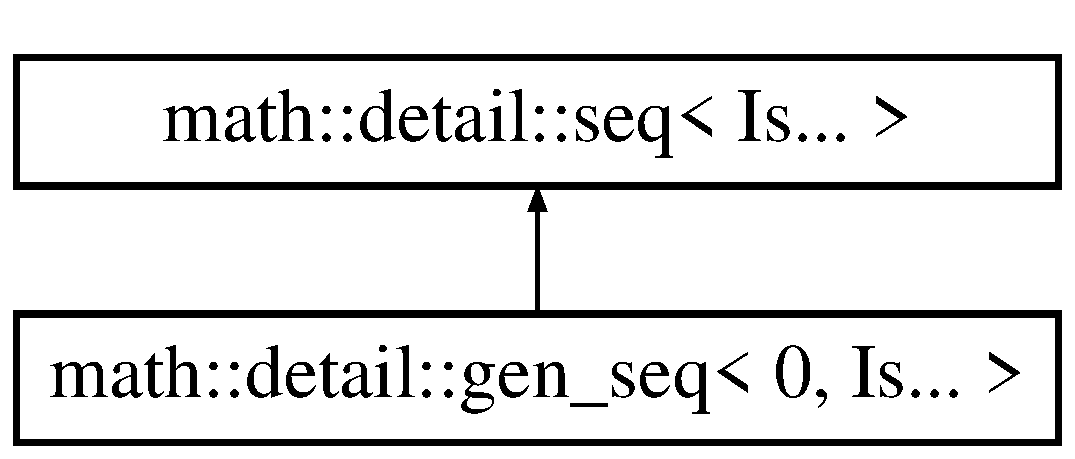
\includegraphics[height=2.000000cm]{structmath_1_1detail_1_1gen__seq_3_010_00_01_is_8_8_8_01_4}
\end{center}
\end{figure}


The documentation for this struct was generated from the following file\+:\begin{DoxyCompactItemize}
\item 
include/\hyperlink{math__constexpr_8h}{math\+\_\+constexpr.\+h}\end{DoxyCompactItemize}

\hypertarget{class_integrate}{}\section{Integrate$<$ order, y\+\_\+type, Polynomial, Quadrature $>$ Class Template Reference}
\label{class_integrate}\index{Integrate$<$ order, y\+\_\+type, Polynomial, Quadrature $>$@{Integrate$<$ order, y\+\_\+type, Polynomial, Quadrature $>$}}


{\ttfamily \#include $<$integrate.\+h$>$}

\subsection*{Public Member Functions}
\begin{DoxyCompactItemize}
\item 
constexpr int \hyperlink{class_integrate_ac76c916feda54370585d288f80802f05}{vmult\+\_\+mass} (std\+::array$<$ std\+::array$<$ y\+\_\+type, order+1 $>$, order+1 $>$ \&y, const std\+::array$<$ std\+::array$<$ y\+\_\+type, order+1 $>$, order+1 $>$ \&u) const
\item 
constexpr int \hyperlink{class_integrate_ae828197f1ebebe1332217481d98c8462}{vmult\+\_\+laplacian} (std\+::array$<$ std\+::array$<$ y\+\_\+type, order+1 $>$, order+1 $>$ \&y, const std\+::array$<$ std\+::array$<$ y\+\_\+type, order+1 $>$, order+1 $>$ \&u) const
\end{DoxyCompactItemize}


\subsection{Member Function Documentation}
\mbox{\Hypertarget{class_integrate_ae828197f1ebebe1332217481d98c8462}\label{class_integrate_ae828197f1ebebe1332217481d98c8462}} 
\index{Integrate@{Integrate}!vmult\+\_\+laplacian@{vmult\+\_\+laplacian}}
\index{vmult\+\_\+laplacian@{vmult\+\_\+laplacian}!Integrate@{Integrate}}
\subsubsection{\texorpdfstring{vmult\+\_\+laplacian()}{vmult\_laplacian()}}
{\footnotesize\ttfamily template$<$int order, typename y\+\_\+type , template$<$ int, typename $>$ class Polynomial, template$<$ int, typename $>$ class Quadrature$>$ \\
constexpr int \hyperlink{class_integrate}{Integrate}$<$ order, y\+\_\+type, \hyperlink{class_polynomial}{Polynomial}, \hyperlink{class_quadrature}{Quadrature} $>$\+::vmult\+\_\+laplacian (\begin{DoxyParamCaption}\item[{std\+::array$<$ std\+::array$<$ y\+\_\+type, order+1 $>$, order+1 $>$ \&}]{y,  }\item[{const std\+::array$<$ std\+::array$<$ y\+\_\+type, order+1 $>$, order+1 $>$ \&}]{u }\end{DoxyParamCaption}) const\hspace{0.3cm}{\ttfamily [inline]}}

\mbox{\Hypertarget{class_integrate_ac76c916feda54370585d288f80802f05}\label{class_integrate_ac76c916feda54370585d288f80802f05}} 
\index{Integrate@{Integrate}!vmult\+\_\+mass@{vmult\+\_\+mass}}
\index{vmult\+\_\+mass@{vmult\+\_\+mass}!Integrate@{Integrate}}
\subsubsection{\texorpdfstring{vmult\+\_\+mass()}{vmult\_mass()}}
{\footnotesize\ttfamily template$<$int order, typename y\+\_\+type , template$<$ int, typename $>$ class Polynomial, template$<$ int, typename $>$ class Quadrature$>$ \\
constexpr int \hyperlink{class_integrate}{Integrate}$<$ order, y\+\_\+type, \hyperlink{class_polynomial}{Polynomial}, \hyperlink{class_quadrature}{Quadrature} $>$\+::vmult\+\_\+mass (\begin{DoxyParamCaption}\item[{std\+::array$<$ std\+::array$<$ y\+\_\+type, order+1 $>$, order+1 $>$ \&}]{y,  }\item[{const std\+::array$<$ std\+::array$<$ y\+\_\+type, order+1 $>$, order+1 $>$ \&}]{u }\end{DoxyParamCaption}) const\hspace{0.3cm}{\ttfamily [inline]}}



The documentation for this class was generated from the following file\+:\begin{DoxyCompactItemize}
\item 
include/\hyperlink{integrate_8h}{integrate.\+h}\end{DoxyCompactItemize}

\hypertarget{class_polynomial}{}\section{Polynomial$<$ order, y\+\_\+type, Quadrature $>$ Class Template Reference}
\label{class_polynomial}\index{Polynomial$<$ order, y\+\_\+type, Quadrature $>$@{Polynomial$<$ order, y\+\_\+type, Quadrature $>$}}


{\ttfamily \#include $<$polynomial.\+h$>$}

\subsection*{Public Member Functions}
\begin{DoxyCompactItemize}
\item 
constexpr \hyperlink{class_polynomial_a00671b3dba3b832c130d1f019c7702c3}{Polynomial} ()
\item 
constexpr \hyperlink{classconstexpr__array}{constexpr\+\_\+array}$<$ y\+\_\+type, order+1 $>$ \hyperlink{class_polynomial_a231fb6b5f655784af1628e9b2f261f08}{compute\+\_\+knots} () const
\item 
{\footnotesize template$<$y\+\_\+type $\ast$ x, unsigned int i$>$ }\\constexpr y\+\_\+type \hyperlink{class_polynomial_a045b1955cf3f6dda4db8b1b50048ab5b}{eval\+\_\+lagrange} () const
\item 
{\footnotesize template$<$y\+\_\+type $\ast$ x, unsigned int i$>$ }\\constexpr y\+\_\+type \hyperlink{class_polynomial_abd8ecf134802a11d3bd286a778b5772c}{eval\+\_\+1st\+\_\+derivative} () const
\item 
{\footnotesize template$<$y\+\_\+type $\ast$ x, unsigned int i$>$ }\\constexpr y\+\_\+type \hyperlink{class_polynomial_a8f135c739984908c26dd9c6dbe045614}{eval\+\_\+2nd\+\_\+derivative} () const
\end{DoxyCompactItemize}
\subsection*{Public Attributes}
\begin{DoxyCompactItemize}
\item 
const \hyperlink{classconstexpr__array}{constexpr\+\_\+array}$<$ y\+\_\+type, order+1 $>$ \hyperlink{class_polynomial_a4319b08af5d88c22598210920ef74d7d}{knots}
\end{DoxyCompactItemize}


\subsection{Constructor \& Destructor Documentation}
\mbox{\Hypertarget{class_polynomial_a00671b3dba3b832c130d1f019c7702c3}\label{class_polynomial_a00671b3dba3b832c130d1f019c7702c3}} 
\index{Polynomial@{Polynomial}!Polynomial@{Polynomial}}
\index{Polynomial@{Polynomial}!Polynomial@{Polynomial}}
\subsubsection{\texorpdfstring{Polynomial()}{Polynomial()}}
{\footnotesize\ttfamily template$<$size\+\_\+t order, typename y\+\_\+type, template$<$ typename, size\+\_\+t $>$ class Quadrature$>$ \\
constexpr \hyperlink{class_polynomial}{Polynomial}$<$ order, y\+\_\+type, \hyperlink{class_quadrature}{Quadrature} $>$\+::\hyperlink{class_polynomial}{Polynomial} (\begin{DoxyParamCaption}{ }\end{DoxyParamCaption})\hspace{0.3cm}{\ttfamily [inline]}}



\subsection{Member Function Documentation}
\mbox{\Hypertarget{class_polynomial_a231fb6b5f655784af1628e9b2f261f08}\label{class_polynomial_a231fb6b5f655784af1628e9b2f261f08}} 
\index{Polynomial@{Polynomial}!compute\+\_\+knots@{compute\+\_\+knots}}
\index{compute\+\_\+knots@{compute\+\_\+knots}!Polynomial@{Polynomial}}
\subsubsection{\texorpdfstring{compute\+\_\+knots()}{compute\_knots()}}
{\footnotesize\ttfamily template$<$size\+\_\+t order, typename y\+\_\+type, template$<$ typename, size\+\_\+t $>$ class Quadrature$>$ \\
constexpr \hyperlink{classconstexpr__array}{constexpr\+\_\+array}$<$y\+\_\+type, order + 1$>$ \hyperlink{class_polynomial}{Polynomial}$<$ order, y\+\_\+type, \hyperlink{class_quadrature}{Quadrature} $>$\+::compute\+\_\+knots (\begin{DoxyParamCaption}{ }\end{DoxyParamCaption}) const\hspace{0.3cm}{\ttfamily [inline]}}

\mbox{\Hypertarget{class_polynomial_abd8ecf134802a11d3bd286a778b5772c}\label{class_polynomial_abd8ecf134802a11d3bd286a778b5772c}} 
\index{Polynomial@{Polynomial}!eval\+\_\+1st\+\_\+derivative@{eval\+\_\+1st\+\_\+derivative}}
\index{eval\+\_\+1st\+\_\+derivative@{eval\+\_\+1st\+\_\+derivative}!Polynomial@{Polynomial}}
\subsubsection{\texorpdfstring{eval\+\_\+1st\+\_\+derivative()}{eval\_1st\_derivative()}}
{\footnotesize\ttfamily template$<$size\+\_\+t order, typename y\+\_\+type, template$<$ typename, size\+\_\+t $>$ class Quadrature$>$ \\
template$<$y\+\_\+type $\ast$ x, unsigned int i$>$ \\
constexpr y\+\_\+type \hyperlink{class_polynomial}{Polynomial}$<$ order, y\+\_\+type, \hyperlink{class_quadrature}{Quadrature} $>$\+::eval\+\_\+1st\+\_\+derivative (\begin{DoxyParamCaption}{ }\end{DoxyParamCaption}) const\hspace{0.3cm}{\ttfamily [inline]}}

\mbox{\Hypertarget{class_polynomial_a8f135c739984908c26dd9c6dbe045614}\label{class_polynomial_a8f135c739984908c26dd9c6dbe045614}} 
\index{Polynomial@{Polynomial}!eval\+\_\+2nd\+\_\+derivative@{eval\+\_\+2nd\+\_\+derivative}}
\index{eval\+\_\+2nd\+\_\+derivative@{eval\+\_\+2nd\+\_\+derivative}!Polynomial@{Polynomial}}
\subsubsection{\texorpdfstring{eval\+\_\+2nd\+\_\+derivative()}{eval\_2nd\_derivative()}}
{\footnotesize\ttfamily template$<$size\+\_\+t order, typename y\+\_\+type, template$<$ typename, size\+\_\+t $>$ class Quadrature$>$ \\
template$<$y\+\_\+type $\ast$ x, unsigned int i$>$ \\
constexpr y\+\_\+type \hyperlink{class_polynomial}{Polynomial}$<$ order, y\+\_\+type, \hyperlink{class_quadrature}{Quadrature} $>$\+::eval\+\_\+2nd\+\_\+derivative (\begin{DoxyParamCaption}{ }\end{DoxyParamCaption}) const\hspace{0.3cm}{\ttfamily [inline]}}

\mbox{\Hypertarget{class_polynomial_a045b1955cf3f6dda4db8b1b50048ab5b}\label{class_polynomial_a045b1955cf3f6dda4db8b1b50048ab5b}} 
\index{Polynomial@{Polynomial}!eval\+\_\+lagrange@{eval\+\_\+lagrange}}
\index{eval\+\_\+lagrange@{eval\+\_\+lagrange}!Polynomial@{Polynomial}}
\subsubsection{\texorpdfstring{eval\+\_\+lagrange()}{eval\_lagrange()}}
{\footnotesize\ttfamily template$<$size\+\_\+t order, typename y\+\_\+type, template$<$ typename, size\+\_\+t $>$ class Quadrature$>$ \\
template$<$y\+\_\+type $\ast$ x, unsigned int i$>$ \\
constexpr y\+\_\+type \hyperlink{class_polynomial}{Polynomial}$<$ order, y\+\_\+type, \hyperlink{class_quadrature}{Quadrature} $>$\+::eval\+\_\+lagrange (\begin{DoxyParamCaption}{ }\end{DoxyParamCaption}) const\hspace{0.3cm}{\ttfamily [inline]}}



\subsection{Member Data Documentation}
\mbox{\Hypertarget{class_polynomial_a4319b08af5d88c22598210920ef74d7d}\label{class_polynomial_a4319b08af5d88c22598210920ef74d7d}} 
\index{Polynomial@{Polynomial}!knots@{knots}}
\index{knots@{knots}!Polynomial@{Polynomial}}
\subsubsection{\texorpdfstring{knots}{knots}}
{\footnotesize\ttfamily template$<$size\+\_\+t order, typename y\+\_\+type, template$<$ typename, size\+\_\+t $>$ class Quadrature$>$ \\
const \hyperlink{classconstexpr__array}{constexpr\+\_\+array}$<$y\+\_\+type, order+1$>$ \hyperlink{class_polynomial}{Polynomial}$<$ order, y\+\_\+type, \hyperlink{class_quadrature}{Quadrature} $>$\+::knots}



The documentation for this class was generated from the following file\+:\begin{DoxyCompactItemize}
\item 
include/\hyperlink{polynomial_8h}{polynomial.\+h}\end{DoxyCompactItemize}

\hypertarget{class_quadrature}{}\section{Quadrature$<$ y\+\_\+type, order $>$ Class Template Reference}
\label{class_quadrature}\index{Quadrature$<$ y\+\_\+type, order $>$@{Quadrature$<$ y\+\_\+type, order $>$}}


{\ttfamily \#include $<$quadrature\+\_\+constexpr.\+h$>$}

\subsection*{Public Member Functions}
\begin{DoxyCompactItemize}
\item 
constexpr \hyperlink{class_quadrature_a0856d3ef4be07d572fd94d34f60ae6cb}{Quadrature} ()
\item 
constexpr const y\+\_\+type \& \hyperlink{class_quadrature_a99f64a4cef3011cbf0df06a4e8eec0c0}{operator\mbox{[}$\,$\mbox{]}} (size\+\_\+t n) const
\item 
constexpr y\+\_\+type \hyperlink{class_quadrature_a58f654e4f2cc08855dfed52d65b35c04}{sin\+\_\+input} (int i, int m) const
\item 
{\footnotesize template$<$size\+\_\+t n$>$ }\\constexpr y\+\_\+type \hyperlink{class_quadrature_a14035efb920cf6ab00fae290e5bbe4bf}{JacobiP} (y\+\_\+type x, int alpha, int beta) const
\item 
constexpr \hyperlink{classconstexpr__array}{constexpr\+\_\+array}$<$ y\+\_\+type, order+1 $>$ \hyperlink{class_quadrature_a9c99c8f4086eec3e94e0eae8a50506ff}{compute\+\_\+quadrature\+\_\+points} () const
\item 
constexpr \hyperlink{classconstexpr__array}{constexpr\+\_\+array}$<$ y\+\_\+type, order+1 $>$ \hyperlink{class_quadrature_a904e3b1cad3b304b500701354b30e194}{compute\+\_\+quadrature\+\_\+weights} () const
\item 
{\footnotesize template$<$size\+\_\+t n$>$ }\\constexpr y\+\_\+type \hyperlink{class_quadrature_ad361ff7a9bfdb5721a107341abfb37d4}{gamma} () const
\item 
constexpr y\+\_\+type \hyperlink{class_quadrature_a924d121900f371d20e84fb3d5277ba4d}{compute\+\_\+kth\+\_\+entry} (const unsigned int k, const \hyperlink{classconstexpr__array}{constexpr\+\_\+array}$<$ y\+\_\+type, order+1 $>$ \&knots) const
\item 
constexpr y\+\_\+type \hyperlink{class_quadrature_a760b6b2c4560afa7218533136a00d0ed}{transform\+\_\+kth\+\_\+entry} (const unsigned int k, const \hyperlink{classconstexpr__array}{constexpr\+\_\+array}$<$ y\+\_\+type, order+1 $>$ \&knots) const
\item 
constexpr y\+\_\+type \hyperlink{class_quadrature_a98b32f58c1a69d2430e2ed14283b07e9}{inv\+\_\+transform\+\_\+kth\+\_\+entry} (const unsigned int k, const \hyperlink{classconstexpr__array}{constexpr\+\_\+array}$<$ y\+\_\+type, order+1 $>$ \&knots) const
\end{DoxyCompactItemize}
\subsection*{Public Attributes}
\begin{DoxyCompactItemize}
\item 
const \hyperlink{classconstexpr__array}{constexpr\+\_\+array}$<$ y\+\_\+type, order+1 $>$ \hyperlink{class_quadrature_ac953b6311f9120fd2c0d8e5bc0d47a8a}{knots\+\_\+}
\item 
const \hyperlink{classconstexpr__array}{constexpr\+\_\+array}$<$ y\+\_\+type, order+1 $>$ \hyperlink{class_quadrature_a333f9daea5b493b74ded779ae4a7c8c9}{weights\+\_\+}
\end{DoxyCompactItemize}


\subsection{Constructor \& Destructor Documentation}
\mbox{\Hypertarget{class_quadrature_a0856d3ef4be07d572fd94d34f60ae6cb}\label{class_quadrature_a0856d3ef4be07d572fd94d34f60ae6cb}} 
\index{Quadrature@{Quadrature}!Quadrature@{Quadrature}}
\index{Quadrature@{Quadrature}!Quadrature@{Quadrature}}
\subsubsection{\texorpdfstring{Quadrature()}{Quadrature()}}
{\footnotesize\ttfamily template$<$typename y\+\_\+type, size\+\_\+t order$>$ \\
constexpr \hyperlink{class_quadrature}{Quadrature}$<$ y\+\_\+type, order $>$\+::\hyperlink{class_quadrature}{Quadrature} (\begin{DoxyParamCaption}{ }\end{DoxyParamCaption})\hspace{0.3cm}{\ttfamily [inline]}}



\subsection{Member Function Documentation}
\mbox{\Hypertarget{class_quadrature_a924d121900f371d20e84fb3d5277ba4d}\label{class_quadrature_a924d121900f371d20e84fb3d5277ba4d}} 
\index{Quadrature@{Quadrature}!compute\+\_\+kth\+\_\+entry@{compute\+\_\+kth\+\_\+entry}}
\index{compute\+\_\+kth\+\_\+entry@{compute\+\_\+kth\+\_\+entry}!Quadrature@{Quadrature}}
\subsubsection{\texorpdfstring{compute\+\_\+kth\+\_\+entry()}{compute\_kth\_entry()}}
{\footnotesize\ttfamily template$<$typename y\+\_\+type, size\+\_\+t order$>$ \\
constexpr y\+\_\+type \hyperlink{class_quadrature}{Quadrature}$<$ y\+\_\+type, order $>$\+::compute\+\_\+kth\+\_\+entry (\begin{DoxyParamCaption}\item[{const unsigned int}]{k,  }\item[{const \hyperlink{classconstexpr__array}{constexpr\+\_\+array}$<$ y\+\_\+type, order+1 $>$ \&}]{knots }\end{DoxyParamCaption}) const\hspace{0.3cm}{\ttfamily [inline]}}

\mbox{\Hypertarget{class_quadrature_a9c99c8f4086eec3e94e0eae8a50506ff}\label{class_quadrature_a9c99c8f4086eec3e94e0eae8a50506ff}} 
\index{Quadrature@{Quadrature}!compute\+\_\+quadrature\+\_\+points@{compute\+\_\+quadrature\+\_\+points}}
\index{compute\+\_\+quadrature\+\_\+points@{compute\+\_\+quadrature\+\_\+points}!Quadrature@{Quadrature}}
\subsubsection{\texorpdfstring{compute\+\_\+quadrature\+\_\+points()}{compute\_quadrature\_points()}}
{\footnotesize\ttfamily template$<$typename y\+\_\+type, size\+\_\+t order$>$ \\
constexpr \hyperlink{classconstexpr__array}{constexpr\+\_\+array}$<$ y\+\_\+type, order + 1 $>$ \hyperlink{class_quadrature}{Quadrature}$<$ y\+\_\+type, order $>$\+::compute\+\_\+quadrature\+\_\+points (\begin{DoxyParamCaption}{ }\end{DoxyParamCaption}) const\hspace{0.3cm}{\ttfamily [inline]}}

\mbox{\Hypertarget{class_quadrature_a904e3b1cad3b304b500701354b30e194}\label{class_quadrature_a904e3b1cad3b304b500701354b30e194}} 
\index{Quadrature@{Quadrature}!compute\+\_\+quadrature\+\_\+weights@{compute\+\_\+quadrature\+\_\+weights}}
\index{compute\+\_\+quadrature\+\_\+weights@{compute\+\_\+quadrature\+\_\+weights}!Quadrature@{Quadrature}}
\subsubsection{\texorpdfstring{compute\+\_\+quadrature\+\_\+weights()}{compute\_quadrature\_weights()}}
{\footnotesize\ttfamily template$<$typename y\+\_\+type, size\+\_\+t order$>$ \\
constexpr \hyperlink{classconstexpr__array}{constexpr\+\_\+array}$<$y\+\_\+type, order + 1$>$ \hyperlink{class_quadrature}{Quadrature}$<$ y\+\_\+type, order $>$\+::compute\+\_\+quadrature\+\_\+weights (\begin{DoxyParamCaption}{ }\end{DoxyParamCaption}) const\hspace{0.3cm}{\ttfamily [inline]}}

\mbox{\Hypertarget{class_quadrature_ad361ff7a9bfdb5721a107341abfb37d4}\label{class_quadrature_ad361ff7a9bfdb5721a107341abfb37d4}} 
\index{Quadrature@{Quadrature}!gamma@{gamma}}
\index{gamma@{gamma}!Quadrature@{Quadrature}}
\subsubsection{\texorpdfstring{gamma()}{gamma()}}
{\footnotesize\ttfamily template$<$typename y\+\_\+type, size\+\_\+t order$>$ \\
template$<$size\+\_\+t n$>$ \\
constexpr y\+\_\+type \hyperlink{class_quadrature}{Quadrature}$<$ y\+\_\+type, order $>$\+::gamma (\begin{DoxyParamCaption}{ }\end{DoxyParamCaption}) const\hspace{0.3cm}{\ttfamily [inline]}}

\mbox{\Hypertarget{class_quadrature_a98b32f58c1a69d2430e2ed14283b07e9}\label{class_quadrature_a98b32f58c1a69d2430e2ed14283b07e9}} 
\index{Quadrature@{Quadrature}!inv\+\_\+transform\+\_\+kth\+\_\+entry@{inv\+\_\+transform\+\_\+kth\+\_\+entry}}
\index{inv\+\_\+transform\+\_\+kth\+\_\+entry@{inv\+\_\+transform\+\_\+kth\+\_\+entry}!Quadrature@{Quadrature}}
\subsubsection{\texorpdfstring{inv\+\_\+transform\+\_\+kth\+\_\+entry()}{inv\_transform\_kth\_entry()}}
{\footnotesize\ttfamily template$<$typename y\+\_\+type, size\+\_\+t order$>$ \\
constexpr y\+\_\+type \hyperlink{class_quadrature}{Quadrature}$<$ y\+\_\+type, order $>$\+::inv\+\_\+transform\+\_\+kth\+\_\+entry (\begin{DoxyParamCaption}\item[{const unsigned int}]{k,  }\item[{const \hyperlink{classconstexpr__array}{constexpr\+\_\+array}$<$ y\+\_\+type, order+1 $>$ \&}]{knots }\end{DoxyParamCaption}) const\hspace{0.3cm}{\ttfamily [inline]}}

\mbox{\Hypertarget{class_quadrature_a14035efb920cf6ab00fae290e5bbe4bf}\label{class_quadrature_a14035efb920cf6ab00fae290e5bbe4bf}} 
\index{Quadrature@{Quadrature}!JacobiP@{JacobiP}}
\index{JacobiP@{JacobiP}!Quadrature@{Quadrature}}
\subsubsection{\texorpdfstring{Jacobi\+P()}{JacobiP()}}
{\footnotesize\ttfamily template$<$typename y\+\_\+type, size\+\_\+t order$>$ \\
template$<$size\+\_\+t n$>$ \\
constexpr y\+\_\+type \hyperlink{class_quadrature}{Quadrature}$<$ y\+\_\+type, order $>$\+::JacobiP (\begin{DoxyParamCaption}\item[{y\+\_\+type}]{x,  }\item[{int}]{alpha,  }\item[{int}]{beta }\end{DoxyParamCaption}) const\hspace{0.3cm}{\ttfamily [inline]}}

\mbox{\Hypertarget{class_quadrature_a99f64a4cef3011cbf0df06a4e8eec0c0}\label{class_quadrature_a99f64a4cef3011cbf0df06a4e8eec0c0}} 
\index{Quadrature@{Quadrature}!operator\mbox{[}\mbox{]}@{operator[]}}
\index{operator\mbox{[}\mbox{]}@{operator[]}!Quadrature@{Quadrature}}
\subsubsection{\texorpdfstring{operator[]()}{operator[]()}}
{\footnotesize\ttfamily template$<$typename y\+\_\+type, size\+\_\+t order$>$ \\
constexpr const y\+\_\+type\& \hyperlink{class_quadrature}{Quadrature}$<$ y\+\_\+type, order $>$\+::operator\mbox{[}$\,$\mbox{]} (\begin{DoxyParamCaption}\item[{size\+\_\+t}]{n }\end{DoxyParamCaption}) const\hspace{0.3cm}{\ttfamily [inline]}}

\mbox{\Hypertarget{class_quadrature_a58f654e4f2cc08855dfed52d65b35c04}\label{class_quadrature_a58f654e4f2cc08855dfed52d65b35c04}} 
\index{Quadrature@{Quadrature}!sin\+\_\+input@{sin\+\_\+input}}
\index{sin\+\_\+input@{sin\+\_\+input}!Quadrature@{Quadrature}}
\subsubsection{\texorpdfstring{sin\+\_\+input()}{sin\_input()}}
{\footnotesize\ttfamily template$<$typename y\+\_\+type, size\+\_\+t order$>$ \\
constexpr y\+\_\+type \hyperlink{class_quadrature}{Quadrature}$<$ y\+\_\+type, order $>$\+::sin\+\_\+input (\begin{DoxyParamCaption}\item[{int}]{i,  }\item[{int}]{m }\end{DoxyParamCaption}) const\hspace{0.3cm}{\ttfamily [inline]}}

\mbox{\Hypertarget{class_quadrature_a760b6b2c4560afa7218533136a00d0ed}\label{class_quadrature_a760b6b2c4560afa7218533136a00d0ed}} 
\index{Quadrature@{Quadrature}!transform\+\_\+kth\+\_\+entry@{transform\+\_\+kth\+\_\+entry}}
\index{transform\+\_\+kth\+\_\+entry@{transform\+\_\+kth\+\_\+entry}!Quadrature@{Quadrature}}
\subsubsection{\texorpdfstring{transform\+\_\+kth\+\_\+entry()}{transform\_kth\_entry()}}
{\footnotesize\ttfamily template$<$typename y\+\_\+type, size\+\_\+t order$>$ \\
constexpr y\+\_\+type \hyperlink{class_quadrature}{Quadrature}$<$ y\+\_\+type, order $>$\+::transform\+\_\+kth\+\_\+entry (\begin{DoxyParamCaption}\item[{const unsigned int}]{k,  }\item[{const \hyperlink{classconstexpr__array}{constexpr\+\_\+array}$<$ y\+\_\+type, order+1 $>$ \&}]{knots }\end{DoxyParamCaption}) const\hspace{0.3cm}{\ttfamily [inline]}}



\subsection{Member Data Documentation}
\mbox{\Hypertarget{class_quadrature_ac953b6311f9120fd2c0d8e5bc0d47a8a}\label{class_quadrature_ac953b6311f9120fd2c0d8e5bc0d47a8a}} 
\index{Quadrature@{Quadrature}!knots\+\_\+@{knots\+\_\+}}
\index{knots\+\_\+@{knots\+\_\+}!Quadrature@{Quadrature}}
\subsubsection{\texorpdfstring{knots\+\_\+}{knots\_}}
{\footnotesize\ttfamily template$<$typename y\+\_\+type, size\+\_\+t order$>$ \\
const \hyperlink{classconstexpr__array}{constexpr\+\_\+array}$<$ y\+\_\+type, order + 1 $>$ \hyperlink{class_quadrature}{Quadrature}$<$ y\+\_\+type, order $>$\+::knots\+\_\+}

\mbox{\Hypertarget{class_quadrature_a333f9daea5b493b74ded779ae4a7c8c9}\label{class_quadrature_a333f9daea5b493b74ded779ae4a7c8c9}} 
\index{Quadrature@{Quadrature}!weights\+\_\+@{weights\+\_\+}}
\index{weights\+\_\+@{weights\+\_\+}!Quadrature@{Quadrature}}
\subsubsection{\texorpdfstring{weights\+\_\+}{weights\_}}
{\footnotesize\ttfamily template$<$typename y\+\_\+type, size\+\_\+t order$>$ \\
const \hyperlink{classconstexpr__array}{constexpr\+\_\+array}$<$ y\+\_\+type, order + 1 $>$ \hyperlink{class_quadrature}{Quadrature}$<$ y\+\_\+type, order $>$\+::weights\+\_\+}



The documentation for this class was generated from the following file\+:\begin{DoxyCompactItemize}
\item 
include/\hyperlink{quadrature__constexpr_8h}{quadrature\+\_\+constexpr.\+h}\end{DoxyCompactItemize}

\hypertarget{structmath_1_1detail_1_1seq}{}\section{math\+:\+:detail\+:\+:seq$<$ Is $>$ Struct Template Reference}
\label{structmath_1_1detail_1_1seq}\index{math\+::detail\+::seq$<$ Is $>$@{math\+::detail\+::seq$<$ Is $>$}}


{\ttfamily \#include $<$math\+\_\+constexpr.\+h$>$}



The documentation for this struct was generated from the following file\+:\begin{DoxyCompactItemize}
\item 
include/\hyperlink{math__constexpr_8h}{math\+\_\+constexpr.\+h}\end{DoxyCompactItemize}

\hypertarget{structmath_1_1detail_1_1sin__coeffs}{}\section{math\+:\+:detail\+:\+:sin\+\_\+coeffs$<$ T, N $>$ Struct Template Reference}
\label{structmath_1_1detail_1_1sin__coeffs}\index{math\+::detail\+::sin\+\_\+coeffs$<$ T, N $>$@{math\+::detail\+::sin\+\_\+coeffs$<$ T, N $>$}}


{\ttfamily \#include $<$math\+\_\+constexpr.\+h$>$}

\subsection*{Public Types}
\begin{DoxyCompactItemize}
\item 
using \hyperlink{structmath_1_1detail_1_1sin__coeffs_a6d08252591f05c40e48bf7931b2eb135}{array\+\_\+type} = std\+::array$<$ T, N $>$
\end{DoxyCompactItemize}
\subsection*{Static Public Member Functions}
\begin{DoxyCompactItemize}
\item 
static constexpr T \hyperlink{structmath_1_1detail_1_1sin__coeffs_ad40f7e723b43aa410e3c260604ae4cac}{coeff} (std\+::size\+\_\+t n)
\item 
{\footnotesize template$<$std\+::size\+\_\+t... NS$>$ }\\static constexpr \hyperlink{structmath_1_1detail_1_1sin__coeffs_a6d08252591f05c40e48bf7931b2eb135}{array\+\_\+type} \hyperlink{structmath_1_1detail_1_1sin__coeffs_a1c5e8b54d12b2320c994c4eaf7b69b61}{\+\_\+coeffs} (\hyperlink{structmath_1_1detail_1_1seq}{seq}$<$ N\+S... $>$)
\end{DoxyCompactItemize}
\subsection*{Static Public Attributes}
\begin{DoxyCompactItemize}
\item 
static constexpr \hyperlink{structmath_1_1detail_1_1sin__coeffs_a6d08252591f05c40e48bf7931b2eb135}{array\+\_\+type} \hyperlink{structmath_1_1detail_1_1sin__coeffs_a78da0b0c2db5a2c060633a296a21dcc8}{coeffs} =\hyperlink{structmath_1_1detail_1_1sin__coeffs_a1c5e8b54d12b2320c994c4eaf7b69b61}{\+\_\+coeffs}(\hyperlink{structmath_1_1detail_1_1gen__seq}{gen\+\_\+seq}$<$N$>$\{\})
\end{DoxyCompactItemize}


\subsection{Member Typedef Documentation}
\mbox{\Hypertarget{structmath_1_1detail_1_1sin__coeffs_a6d08252591f05c40e48bf7931b2eb135}\label{structmath_1_1detail_1_1sin__coeffs_a6d08252591f05c40e48bf7931b2eb135}} 
\index{math\+::detail\+::sin\+\_\+coeffs@{math\+::detail\+::sin\+\_\+coeffs}!array\+\_\+type@{array\+\_\+type}}
\index{array\+\_\+type@{array\+\_\+type}!math\+::detail\+::sin\+\_\+coeffs@{math\+::detail\+::sin\+\_\+coeffs}}
\subsubsection{\texorpdfstring{array\+\_\+type}{array\_type}}
{\footnotesize\ttfamily template$<$class T , std\+::size\+\_\+t N$>$ \\
using \hyperlink{structmath_1_1detail_1_1sin__coeffs}{math\+::detail\+::sin\+\_\+coeffs}$<$ T, N $>$\+::\hyperlink{structmath_1_1detail_1_1sin__coeffs_a6d08252591f05c40e48bf7931b2eb135}{array\+\_\+type} =  std\+::array$<$T,N$>$}



\subsection{Member Function Documentation}
\mbox{\Hypertarget{structmath_1_1detail_1_1sin__coeffs_a1c5e8b54d12b2320c994c4eaf7b69b61}\label{structmath_1_1detail_1_1sin__coeffs_a1c5e8b54d12b2320c994c4eaf7b69b61}} 
\index{math\+::detail\+::sin\+\_\+coeffs@{math\+::detail\+::sin\+\_\+coeffs}!\+\_\+coeffs@{\+\_\+coeffs}}
\index{\+\_\+coeffs@{\+\_\+coeffs}!math\+::detail\+::sin\+\_\+coeffs@{math\+::detail\+::sin\+\_\+coeffs}}
\subsubsection{\texorpdfstring{\+\_\+coeffs()}{\_coeffs()}}
{\footnotesize\ttfamily template$<$class T , std\+::size\+\_\+t N$>$ \\
template$<$std\+::size\+\_\+t... NS$>$ \\
static constexpr \hyperlink{structmath_1_1detail_1_1sin__coeffs_a6d08252591f05c40e48bf7931b2eb135}{array\+\_\+type} \hyperlink{structmath_1_1detail_1_1sin__coeffs}{math\+::detail\+::sin\+\_\+coeffs}$<$ T, N $>$\+::\+\_\+coeffs (\begin{DoxyParamCaption}\item[{\hyperlink{structmath_1_1detail_1_1seq}{seq}$<$ N\+S... $>$}]{ }\end{DoxyParamCaption})\hspace{0.3cm}{\ttfamily [inline]}, {\ttfamily [static]}}

\mbox{\Hypertarget{structmath_1_1detail_1_1sin__coeffs_ad40f7e723b43aa410e3c260604ae4cac}\label{structmath_1_1detail_1_1sin__coeffs_ad40f7e723b43aa410e3c260604ae4cac}} 
\index{math\+::detail\+::sin\+\_\+coeffs@{math\+::detail\+::sin\+\_\+coeffs}!coeff@{coeff}}
\index{coeff@{coeff}!math\+::detail\+::sin\+\_\+coeffs@{math\+::detail\+::sin\+\_\+coeffs}}
\subsubsection{\texorpdfstring{coeff()}{coeff()}}
{\footnotesize\ttfamily template$<$class T , std\+::size\+\_\+t N$>$ \\
static constexpr T \hyperlink{structmath_1_1detail_1_1sin__coeffs}{math\+::detail\+::sin\+\_\+coeffs}$<$ T, N $>$\+::coeff (\begin{DoxyParamCaption}\item[{std\+::size\+\_\+t}]{n }\end{DoxyParamCaption})\hspace{0.3cm}{\ttfamily [inline]}, {\ttfamily [static]}}



\subsection{Member Data Documentation}
\mbox{\Hypertarget{structmath_1_1detail_1_1sin__coeffs_a78da0b0c2db5a2c060633a296a21dcc8}\label{structmath_1_1detail_1_1sin__coeffs_a78da0b0c2db5a2c060633a296a21dcc8}} 
\index{math\+::detail\+::sin\+\_\+coeffs@{math\+::detail\+::sin\+\_\+coeffs}!coeffs@{coeffs}}
\index{coeffs@{coeffs}!math\+::detail\+::sin\+\_\+coeffs@{math\+::detail\+::sin\+\_\+coeffs}}
\subsubsection{\texorpdfstring{coeffs}{coeffs}}
{\footnotesize\ttfamily template$<$class T , std\+::size\+\_\+t N$>$ \\
constexpr \hyperlink{structmath_1_1detail_1_1sin__coeffs_a6d08252591f05c40e48bf7931b2eb135}{array\+\_\+type} \hyperlink{structmath_1_1detail_1_1sin__coeffs}{math\+::detail\+::sin\+\_\+coeffs}$<$ T, N $>$\+::coeffs =\hyperlink{structmath_1_1detail_1_1sin__coeffs_a1c5e8b54d12b2320c994c4eaf7b69b61}{\+\_\+coeffs}(\hyperlink{structmath_1_1detail_1_1gen__seq}{gen\+\_\+seq}$<$N$>$\{\})\hspace{0.3cm}{\ttfamily [static]}}



The documentation for this struct was generated from the following file\+:\begin{DoxyCompactItemize}
\item 
include/\hyperlink{math__constexpr_8h}{math\+\_\+constexpr.\+h}\end{DoxyCompactItemize}

\hypertarget{class_v_m_u_l_t}{}\section{V\+M\+U\+LT$<$ order, q\+\_\+order, c, y\+\_\+type, Polynomial, Quadrature $>$ Class Template Reference}
\label{class_v_m_u_l_t}\index{V\+M\+U\+L\+T$<$ order, q\+\_\+order, c, y\+\_\+type, Polynomial, Quadrature $>$@{V\+M\+U\+L\+T$<$ order, q\+\_\+order, c, y\+\_\+type, Polynomial, Quadrature $>$}}


{\ttfamily \#include $<$vmult.\+h$>$}

\subsection*{Public Member Functions}
\begin{DoxyCompactItemize}
\item 
\hyperlink{class_v_m_u_l_t_a31d73a0a561c27c4443a167950a9c852}{V\+M\+U\+LT} ()
\item 
void \hyperlink{class_v_m_u_l_t_a0d60b90e214cf4e5d35e3b3c1402ccec}{compute\+\_\+basis\+\_\+matrix} ()
\item 
void \hyperlink{class_v_m_u_l_t_a51170ad231bce36f2be50c5198a2aec0}{compute\+\_\+for\+\_\+gradient} ()
\item 
void \hyperlink{class_v_m_u_l_t_add49b6c92921149a92830f2930074aab}{compute\+\_\+for\+\_\+laplacian} ()
\item 
void \hyperlink{class_v_m_u_l_t_ab903e1707daffaf5480c481281f419db}{vmult\+\_\+mass} (std\+::array$<$ std\+::array$<$ y\+\_\+type, order+1 $>$, order+1 $>$ \&y, std\+::array$<$ std\+::array$<$ y\+\_\+type, order+1 $>$, order+1 $>$ \&u)
\item 
void \hyperlink{class_v_m_u_l_t_a722ef0ecb53e27931993425f5514ea8a}{vmult\+\_\+gradient} (std\+::array$<$ std\+::array$<$ y\+\_\+type, order+1 $>$, order+1 $>$ \&y, std\+::array$<$ std\+::array$<$ y\+\_\+type, order+1 $>$, order+1 $>$ \&u)
\item 
constexpr void \hyperlink{class_v_m_u_l_t_a51c70b05d1f6d934470b1f11526cbc80}{vmult\+\_\+laplacian} (std\+::array$<$ std\+::array$<$ y\+\_\+type, order+1 $>$, order+1 $>$ \&y, std\+::array$<$ std\+::array$<$ y\+\_\+type, order+1 $>$, order+1 $>$ \&u)
\end{DoxyCompactItemize}
\subsection*{Public Attributes}
\begin{DoxyCompactItemize}
\item 
\hyperlink{class_quadrature}{Quadrature}$<$ q\+\_\+order, y\+\_\+type $>$ \hyperlink{class_v_m_u_l_t_a4395585e5102243b07c33abc001d1a7a}{quad}
\item 
\hyperlink{class_polynomial}{Polynomial}$<$ order, y\+\_\+type $>$ \hyperlink{class_v_m_u_l_t_ad9e2a7049062262eee02a278aca1da14}{poly}
\item 
std\+::array$<$ std\+::array$<$ y\+\_\+type, q\+\_\+order $>$, order+1 $>$ \hyperlink{class_v_m_u_l_t_a6a9fd7d80d98b790caae6cb72bb6db05}{N\+\_\+\+Transposed}
\item 
std\+::array$<$ std\+::array$<$ y\+\_\+type, order+1 $>$, q\+\_\+order $>$ \hyperlink{class_v_m_u_l_t_ad06ca1f3f261548524b59bd1a6dbe80d}{NW}
\item 
std\+::array$<$ std\+::array$<$ y\+\_\+type, order+1 $>$, order+1 $>$ \hyperlink{class_v_m_u_l_t_a1997e77da014ab5ee4b2c13670845599}{N\+\_\+\+Product}
\item 
std\+::array$<$ std\+::array$<$ y\+\_\+type, q\+\_\+order $>$, order+1 $>$ \hyperlink{class_v_m_u_l_t_a317e137345aaeb4967db30ca7e479435}{Ndx\+\_\+\+Transposed}
\item 
std\+::array$<$ std\+::array$<$ y\+\_\+type, order+1 $>$, q\+\_\+order $>$ \hyperlink{class_v_m_u_l_t_a4fb623e96001cbc01d7289c3465544ec}{N\+Wdx}
\item 
std\+::array$<$ std\+::array$<$ y\+\_\+type, order+1 $>$, order+1 $>$ \hyperlink{class_v_m_u_l_t_a9b41e56739c33dfa1a547b8b0b757d42}{Ndx\+\_\+\+Product}
\item 
std\+::array$<$ std\+::array$<$ y\+\_\+type, q\+\_\+order $>$, order+1 $>$ \hyperlink{class_v_m_u_l_t_a11fec13d3ecba614678ce07a466bdcb1}{Ndxdx\+\_\+\+Transposed}
\item 
std\+::array$<$ std\+::array$<$ y\+\_\+type, order+1 $>$, order+1 $>$ \hyperlink{class_v_m_u_l_t_a74d462b33c24fb447dc7267be3725720}{Ndxdx\+\_\+\+Product}
\end{DoxyCompactItemize}


\subsection{Constructor \& Destructor Documentation}
\mbox{\Hypertarget{class_v_m_u_l_t_a31d73a0a561c27c4443a167950a9c852}\label{class_v_m_u_l_t_a31d73a0a561c27c4443a167950a9c852}} 
\index{V\+M\+U\+LT@{V\+M\+U\+LT}!V\+M\+U\+LT@{V\+M\+U\+LT}}
\index{V\+M\+U\+LT@{V\+M\+U\+LT}!V\+M\+U\+LT@{V\+M\+U\+LT}}
\subsubsection{\texorpdfstring{V\+M\+U\+L\+T()}{VMULT()}}
{\footnotesize\ttfamily template$<$int order, int q\+\_\+order, int c, typename y\+\_\+type , template$<$ int, typename $>$ class Polynomial, template$<$ int, typename $>$ class Quadrature$>$ \\
\hyperlink{class_v_m_u_l_t}{V\+M\+U\+LT}$<$ order, q\+\_\+order, c, y\+\_\+type, \hyperlink{class_polynomial}{Polynomial}, \hyperlink{class_quadrature}{Quadrature} $>$\+::\hyperlink{class_v_m_u_l_t}{V\+M\+U\+LT} (\begin{DoxyParamCaption}{ }\end{DoxyParamCaption})\hspace{0.3cm}{\ttfamily [inline]}}



\subsection{Member Function Documentation}
\mbox{\Hypertarget{class_v_m_u_l_t_a0d60b90e214cf4e5d35e3b3c1402ccec}\label{class_v_m_u_l_t_a0d60b90e214cf4e5d35e3b3c1402ccec}} 
\index{V\+M\+U\+LT@{V\+M\+U\+LT}!compute\+\_\+basis\+\_\+matrix@{compute\+\_\+basis\+\_\+matrix}}
\index{compute\+\_\+basis\+\_\+matrix@{compute\+\_\+basis\+\_\+matrix}!V\+M\+U\+LT@{V\+M\+U\+LT}}
\subsubsection{\texorpdfstring{compute\+\_\+basis\+\_\+matrix()}{compute\_basis\_matrix()}}
{\footnotesize\ttfamily template$<$int order, int q\+\_\+order, int c, typename y\+\_\+type , template$<$ int, typename $>$ class Polynomial, template$<$ int, typename $>$ class Quadrature$>$ \\
void \hyperlink{class_v_m_u_l_t}{V\+M\+U\+LT}$<$ order, q\+\_\+order, c, y\+\_\+type, \hyperlink{class_polynomial}{Polynomial}, \hyperlink{class_quadrature}{Quadrature} $>$\+::compute\+\_\+basis\+\_\+matrix (\begin{DoxyParamCaption}{ }\end{DoxyParamCaption})\hspace{0.3cm}{\ttfamily [inline]}}

\mbox{\Hypertarget{class_v_m_u_l_t_a51170ad231bce36f2be50c5198a2aec0}\label{class_v_m_u_l_t_a51170ad231bce36f2be50c5198a2aec0}} 
\index{V\+M\+U\+LT@{V\+M\+U\+LT}!compute\+\_\+for\+\_\+gradient@{compute\+\_\+for\+\_\+gradient}}
\index{compute\+\_\+for\+\_\+gradient@{compute\+\_\+for\+\_\+gradient}!V\+M\+U\+LT@{V\+M\+U\+LT}}
\subsubsection{\texorpdfstring{compute\+\_\+for\+\_\+gradient()}{compute\_for\_gradient()}}
{\footnotesize\ttfamily template$<$int order, int q\+\_\+order, int c, typename y\+\_\+type , template$<$ int, typename $>$ class Polynomial, template$<$ int, typename $>$ class Quadrature$>$ \\
void \hyperlink{class_v_m_u_l_t}{V\+M\+U\+LT}$<$ order, q\+\_\+order, c, y\+\_\+type, \hyperlink{class_polynomial}{Polynomial}, \hyperlink{class_quadrature}{Quadrature} $>$\+::compute\+\_\+for\+\_\+gradient (\begin{DoxyParamCaption}{ }\end{DoxyParamCaption})\hspace{0.3cm}{\ttfamily [inline]}}

\mbox{\Hypertarget{class_v_m_u_l_t_add49b6c92921149a92830f2930074aab}\label{class_v_m_u_l_t_add49b6c92921149a92830f2930074aab}} 
\index{V\+M\+U\+LT@{V\+M\+U\+LT}!compute\+\_\+for\+\_\+laplacian@{compute\+\_\+for\+\_\+laplacian}}
\index{compute\+\_\+for\+\_\+laplacian@{compute\+\_\+for\+\_\+laplacian}!V\+M\+U\+LT@{V\+M\+U\+LT}}
\subsubsection{\texorpdfstring{compute\+\_\+for\+\_\+laplacian()}{compute\_for\_laplacian()}}
{\footnotesize\ttfamily template$<$int order, int q\+\_\+order, int c, typename y\+\_\+type , template$<$ int, typename $>$ class Polynomial, template$<$ int, typename $>$ class Quadrature$>$ \\
void \hyperlink{class_v_m_u_l_t}{V\+M\+U\+LT}$<$ order, q\+\_\+order, c, y\+\_\+type, \hyperlink{class_polynomial}{Polynomial}, \hyperlink{class_quadrature}{Quadrature} $>$\+::compute\+\_\+for\+\_\+laplacian (\begin{DoxyParamCaption}{ }\end{DoxyParamCaption})\hspace{0.3cm}{\ttfamily [inline]}}

\mbox{\Hypertarget{class_v_m_u_l_t_a722ef0ecb53e27931993425f5514ea8a}\label{class_v_m_u_l_t_a722ef0ecb53e27931993425f5514ea8a}} 
\index{V\+M\+U\+LT@{V\+M\+U\+LT}!vmult\+\_\+gradient@{vmult\+\_\+gradient}}
\index{vmult\+\_\+gradient@{vmult\+\_\+gradient}!V\+M\+U\+LT@{V\+M\+U\+LT}}
\subsubsection{\texorpdfstring{vmult\+\_\+gradient()}{vmult\_gradient()}}
{\footnotesize\ttfamily template$<$int order, int q\+\_\+order, int c, typename y\+\_\+type , template$<$ int, typename $>$ class Polynomial, template$<$ int, typename $>$ class Quadrature$>$ \\
void \hyperlink{class_v_m_u_l_t}{V\+M\+U\+LT}$<$ order, q\+\_\+order, c, y\+\_\+type, \hyperlink{class_polynomial}{Polynomial}, \hyperlink{class_quadrature}{Quadrature} $>$\+::vmult\+\_\+gradient (\begin{DoxyParamCaption}\item[{std\+::array$<$ std\+::array$<$ y\+\_\+type, order+1 $>$, order+1 $>$ \&}]{y,  }\item[{std\+::array$<$ std\+::array$<$ y\+\_\+type, order+1 $>$, order+1 $>$ \&}]{u }\end{DoxyParamCaption})\hspace{0.3cm}{\ttfamily [inline]}}

\mbox{\Hypertarget{class_v_m_u_l_t_a51c70b05d1f6d934470b1f11526cbc80}\label{class_v_m_u_l_t_a51c70b05d1f6d934470b1f11526cbc80}} 
\index{V\+M\+U\+LT@{V\+M\+U\+LT}!vmult\+\_\+laplacian@{vmult\+\_\+laplacian}}
\index{vmult\+\_\+laplacian@{vmult\+\_\+laplacian}!V\+M\+U\+LT@{V\+M\+U\+LT}}
\subsubsection{\texorpdfstring{vmult\+\_\+laplacian()}{vmult\_laplacian()}}
{\footnotesize\ttfamily template$<$int order, int q\+\_\+order, int c, typename y\+\_\+type , template$<$ int, typename $>$ class Polynomial, template$<$ int, typename $>$ class Quadrature$>$ \\
constexpr void \hyperlink{class_v_m_u_l_t}{V\+M\+U\+LT}$<$ order, q\+\_\+order, c, y\+\_\+type, \hyperlink{class_polynomial}{Polynomial}, \hyperlink{class_quadrature}{Quadrature} $>$\+::vmult\+\_\+laplacian (\begin{DoxyParamCaption}\item[{std\+::array$<$ std\+::array$<$ y\+\_\+type, order+1 $>$, order+1 $>$ \&}]{y,  }\item[{std\+::array$<$ std\+::array$<$ y\+\_\+type, order+1 $>$, order+1 $>$ \&}]{u }\end{DoxyParamCaption})\hspace{0.3cm}{\ttfamily [inline]}}

\mbox{\Hypertarget{class_v_m_u_l_t_ab903e1707daffaf5480c481281f419db}\label{class_v_m_u_l_t_ab903e1707daffaf5480c481281f419db}} 
\index{V\+M\+U\+LT@{V\+M\+U\+LT}!vmult\+\_\+mass@{vmult\+\_\+mass}}
\index{vmult\+\_\+mass@{vmult\+\_\+mass}!V\+M\+U\+LT@{V\+M\+U\+LT}}
\subsubsection{\texorpdfstring{vmult\+\_\+mass()}{vmult\_mass()}}
{\footnotesize\ttfamily template$<$int order, int q\+\_\+order, int c, typename y\+\_\+type , template$<$ int, typename $>$ class Polynomial, template$<$ int, typename $>$ class Quadrature$>$ \\
void \hyperlink{class_v_m_u_l_t}{V\+M\+U\+LT}$<$ order, q\+\_\+order, c, y\+\_\+type, \hyperlink{class_polynomial}{Polynomial}, \hyperlink{class_quadrature}{Quadrature} $>$\+::vmult\+\_\+mass (\begin{DoxyParamCaption}\item[{std\+::array$<$ std\+::array$<$ y\+\_\+type, order+1 $>$, order+1 $>$ \&}]{y,  }\item[{std\+::array$<$ std\+::array$<$ y\+\_\+type, order+1 $>$, order+1 $>$ \&}]{u }\end{DoxyParamCaption})\hspace{0.3cm}{\ttfamily [inline]}}



\subsection{Member Data Documentation}
\mbox{\Hypertarget{class_v_m_u_l_t_a1997e77da014ab5ee4b2c13670845599}\label{class_v_m_u_l_t_a1997e77da014ab5ee4b2c13670845599}} 
\index{V\+M\+U\+LT@{V\+M\+U\+LT}!N\+\_\+\+Product@{N\+\_\+\+Product}}
\index{N\+\_\+\+Product@{N\+\_\+\+Product}!V\+M\+U\+LT@{V\+M\+U\+LT}}
\subsubsection{\texorpdfstring{N\+\_\+\+Product}{N\_Product}}
{\footnotesize\ttfamily template$<$int order, int q\+\_\+order, int c, typename y\+\_\+type , template$<$ int, typename $>$ class Polynomial, template$<$ int, typename $>$ class Quadrature$>$ \\
std\+::array$<$ std\+::array $<$y\+\_\+type, order +1$>$, order + 1$>$ \hyperlink{class_v_m_u_l_t}{V\+M\+U\+LT}$<$ order, q\+\_\+order, c, y\+\_\+type, \hyperlink{class_polynomial}{Polynomial}, \hyperlink{class_quadrature}{Quadrature} $>$\+::N\+\_\+\+Product}

\mbox{\Hypertarget{class_v_m_u_l_t_a6a9fd7d80d98b790caae6cb72bb6db05}\label{class_v_m_u_l_t_a6a9fd7d80d98b790caae6cb72bb6db05}} 
\index{V\+M\+U\+LT@{V\+M\+U\+LT}!N\+\_\+\+Transposed@{N\+\_\+\+Transposed}}
\index{N\+\_\+\+Transposed@{N\+\_\+\+Transposed}!V\+M\+U\+LT@{V\+M\+U\+LT}}
\subsubsection{\texorpdfstring{N\+\_\+\+Transposed}{N\_Transposed}}
{\footnotesize\ttfamily template$<$int order, int q\+\_\+order, int c, typename y\+\_\+type , template$<$ int, typename $>$ class Polynomial, template$<$ int, typename $>$ class Quadrature$>$ \\
std\+::array$<$ std\+::array $<$y\+\_\+type, q\+\_\+order$>$, order + 1 $>$ \hyperlink{class_v_m_u_l_t}{V\+M\+U\+LT}$<$ order, q\+\_\+order, c, y\+\_\+type, \hyperlink{class_polynomial}{Polynomial}, \hyperlink{class_quadrature}{Quadrature} $>$\+::N\+\_\+\+Transposed}

\mbox{\Hypertarget{class_v_m_u_l_t_a9b41e56739c33dfa1a547b8b0b757d42}\label{class_v_m_u_l_t_a9b41e56739c33dfa1a547b8b0b757d42}} 
\index{V\+M\+U\+LT@{V\+M\+U\+LT}!Ndx\+\_\+\+Product@{Ndx\+\_\+\+Product}}
\index{Ndx\+\_\+\+Product@{Ndx\+\_\+\+Product}!V\+M\+U\+LT@{V\+M\+U\+LT}}
\subsubsection{\texorpdfstring{Ndx\+\_\+\+Product}{Ndx\_Product}}
{\footnotesize\ttfamily template$<$int order, int q\+\_\+order, int c, typename y\+\_\+type , template$<$ int, typename $>$ class Polynomial, template$<$ int, typename $>$ class Quadrature$>$ \\
std\+::array$<$ std\+::array $<$y\+\_\+type, order +1$>$, order + 1$>$ \hyperlink{class_v_m_u_l_t}{V\+M\+U\+LT}$<$ order, q\+\_\+order, c, y\+\_\+type, \hyperlink{class_polynomial}{Polynomial}, \hyperlink{class_quadrature}{Quadrature} $>$\+::Ndx\+\_\+\+Product}

\mbox{\Hypertarget{class_v_m_u_l_t_a317e137345aaeb4967db30ca7e479435}\label{class_v_m_u_l_t_a317e137345aaeb4967db30ca7e479435}} 
\index{V\+M\+U\+LT@{V\+M\+U\+LT}!Ndx\+\_\+\+Transposed@{Ndx\+\_\+\+Transposed}}
\index{Ndx\+\_\+\+Transposed@{Ndx\+\_\+\+Transposed}!V\+M\+U\+LT@{V\+M\+U\+LT}}
\subsubsection{\texorpdfstring{Ndx\+\_\+\+Transposed}{Ndx\_Transposed}}
{\footnotesize\ttfamily template$<$int order, int q\+\_\+order, int c, typename y\+\_\+type , template$<$ int, typename $>$ class Polynomial, template$<$ int, typename $>$ class Quadrature$>$ \\
std\+::array$<$ std\+::array $<$y\+\_\+type, q\+\_\+order$>$, order + 1 $>$ \hyperlink{class_v_m_u_l_t}{V\+M\+U\+LT}$<$ order, q\+\_\+order, c, y\+\_\+type, \hyperlink{class_polynomial}{Polynomial}, \hyperlink{class_quadrature}{Quadrature} $>$\+::Ndx\+\_\+\+Transposed}

\mbox{\Hypertarget{class_v_m_u_l_t_a74d462b33c24fb447dc7267be3725720}\label{class_v_m_u_l_t_a74d462b33c24fb447dc7267be3725720}} 
\index{V\+M\+U\+LT@{V\+M\+U\+LT}!Ndxdx\+\_\+\+Product@{Ndxdx\+\_\+\+Product}}
\index{Ndxdx\+\_\+\+Product@{Ndxdx\+\_\+\+Product}!V\+M\+U\+LT@{V\+M\+U\+LT}}
\subsubsection{\texorpdfstring{Ndxdx\+\_\+\+Product}{Ndxdx\_Product}}
{\footnotesize\ttfamily template$<$int order, int q\+\_\+order, int c, typename y\+\_\+type , template$<$ int, typename $>$ class Polynomial, template$<$ int, typename $>$ class Quadrature$>$ \\
std\+::array$<$ std\+::array $<$y\+\_\+type, order +1$>$, order + 1$>$ \hyperlink{class_v_m_u_l_t}{V\+M\+U\+LT}$<$ order, q\+\_\+order, c, y\+\_\+type, \hyperlink{class_polynomial}{Polynomial}, \hyperlink{class_quadrature}{Quadrature} $>$\+::Ndxdx\+\_\+\+Product}

\mbox{\Hypertarget{class_v_m_u_l_t_a11fec13d3ecba614678ce07a466bdcb1}\label{class_v_m_u_l_t_a11fec13d3ecba614678ce07a466bdcb1}} 
\index{V\+M\+U\+LT@{V\+M\+U\+LT}!Ndxdx\+\_\+\+Transposed@{Ndxdx\+\_\+\+Transposed}}
\index{Ndxdx\+\_\+\+Transposed@{Ndxdx\+\_\+\+Transposed}!V\+M\+U\+LT@{V\+M\+U\+LT}}
\subsubsection{\texorpdfstring{Ndxdx\+\_\+\+Transposed}{Ndxdx\_Transposed}}
{\footnotesize\ttfamily template$<$int order, int q\+\_\+order, int c, typename y\+\_\+type , template$<$ int, typename $>$ class Polynomial, template$<$ int, typename $>$ class Quadrature$>$ \\
std\+::array$<$ std\+::array $<$y\+\_\+type, q\+\_\+order$>$, order + 1 $>$ \hyperlink{class_v_m_u_l_t}{V\+M\+U\+LT}$<$ order, q\+\_\+order, c, y\+\_\+type, \hyperlink{class_polynomial}{Polynomial}, \hyperlink{class_quadrature}{Quadrature} $>$\+::Ndxdx\+\_\+\+Transposed}

\mbox{\Hypertarget{class_v_m_u_l_t_ad06ca1f3f261548524b59bd1a6dbe80d}\label{class_v_m_u_l_t_ad06ca1f3f261548524b59bd1a6dbe80d}} 
\index{V\+M\+U\+LT@{V\+M\+U\+LT}!NW@{NW}}
\index{NW@{NW}!V\+M\+U\+LT@{V\+M\+U\+LT}}
\subsubsection{\texorpdfstring{NW}{NW}}
{\footnotesize\ttfamily template$<$int order, int q\+\_\+order, int c, typename y\+\_\+type , template$<$ int, typename $>$ class Polynomial, template$<$ int, typename $>$ class Quadrature$>$ \\
std\+::array$<$ std\+::array $<$y\+\_\+type, order + 1$>$, q\+\_\+order $>$ \hyperlink{class_v_m_u_l_t}{V\+M\+U\+LT}$<$ order, q\+\_\+order, c, y\+\_\+type, \hyperlink{class_polynomial}{Polynomial}, \hyperlink{class_quadrature}{Quadrature} $>$\+::NW}

\mbox{\Hypertarget{class_v_m_u_l_t_a4fb623e96001cbc01d7289c3465544ec}\label{class_v_m_u_l_t_a4fb623e96001cbc01d7289c3465544ec}} 
\index{V\+M\+U\+LT@{V\+M\+U\+LT}!N\+Wdx@{N\+Wdx}}
\index{N\+Wdx@{N\+Wdx}!V\+M\+U\+LT@{V\+M\+U\+LT}}
\subsubsection{\texorpdfstring{N\+Wdx}{NWdx}}
{\footnotesize\ttfamily template$<$int order, int q\+\_\+order, int c, typename y\+\_\+type , template$<$ int, typename $>$ class Polynomial, template$<$ int, typename $>$ class Quadrature$>$ \\
std\+::array$<$ std\+::array $<$y\+\_\+type, order + 1$>$, q\+\_\+order $>$ \hyperlink{class_v_m_u_l_t}{V\+M\+U\+LT}$<$ order, q\+\_\+order, c, y\+\_\+type, \hyperlink{class_polynomial}{Polynomial}, \hyperlink{class_quadrature}{Quadrature} $>$\+::N\+Wdx}

\mbox{\Hypertarget{class_v_m_u_l_t_ad9e2a7049062262eee02a278aca1da14}\label{class_v_m_u_l_t_ad9e2a7049062262eee02a278aca1da14}} 
\index{V\+M\+U\+LT@{V\+M\+U\+LT}!poly@{poly}}
\index{poly@{poly}!V\+M\+U\+LT@{V\+M\+U\+LT}}
\subsubsection{\texorpdfstring{poly}{poly}}
{\footnotesize\ttfamily template$<$int order, int q\+\_\+order, int c, typename y\+\_\+type , template$<$ int, typename $>$ class Polynomial, template$<$ int, typename $>$ class Quadrature$>$ \\
\hyperlink{class_polynomial}{Polynomial}$<$order, y\+\_\+type$>$ \hyperlink{class_v_m_u_l_t}{V\+M\+U\+LT}$<$ order, q\+\_\+order, c, y\+\_\+type, \hyperlink{class_polynomial}{Polynomial}, \hyperlink{class_quadrature}{Quadrature} $>$\+::poly}

\mbox{\Hypertarget{class_v_m_u_l_t_a4395585e5102243b07c33abc001d1a7a}\label{class_v_m_u_l_t_a4395585e5102243b07c33abc001d1a7a}} 
\index{V\+M\+U\+LT@{V\+M\+U\+LT}!quad@{quad}}
\index{quad@{quad}!V\+M\+U\+LT@{V\+M\+U\+LT}}
\subsubsection{\texorpdfstring{quad}{quad}}
{\footnotesize\ttfamily template$<$int order, int q\+\_\+order, int c, typename y\+\_\+type , template$<$ int, typename $>$ class Polynomial, template$<$ int, typename $>$ class Quadrature$>$ \\
\hyperlink{class_quadrature}{Quadrature}$<$q\+\_\+order, y\+\_\+type$>$ \hyperlink{class_v_m_u_l_t}{V\+M\+U\+LT}$<$ order, q\+\_\+order, c, y\+\_\+type, \hyperlink{class_polynomial}{Polynomial}, \hyperlink{class_quadrature}{Quadrature} $>$\+::quad}



The documentation for this class was generated from the following file\+:\begin{DoxyCompactItemize}
\item 
include/\hyperlink{vmult_8h}{vmult.\+h}\end{DoxyCompactItemize}

\chapter{File Documentation}
\hypertarget{_c_make_c_compiler_id_8c}{}\section{build/\+C\+Make\+Files/3.7.1/\+Compiler\+Id\+C/\+C\+Make\+C\+Compiler\+Id.c File Reference}
\label{_c_make_c_compiler_id_8c}\index{build/\+C\+Make\+Files/3.\+7.\+1/\+Compiler\+Id\+C/\+C\+Make\+C\+Compiler\+Id.\+c@{build/\+C\+Make\+Files/3.\+7.\+1/\+Compiler\+Id\+C/\+C\+Make\+C\+Compiler\+Id.\+c}}
\subsection*{Macros}
\begin{DoxyCompactItemize}
\item 
\#define \hyperlink{_c_make_c_compiler_id_8c_a81dee0709ded976b2e0319239f72d174}{C\+O\+M\+P\+I\+L\+E\+R\+\_\+\+ID}~\char`\"{}\char`\"{}
\item 
\#define \hyperlink{_c_make_c_compiler_id_8c_a2ae9b72bb13abaabfcf2ee0ba7d3fa1d}{S\+T\+R\+I\+N\+G\+I\+F\+Y\+\_\+\+H\+E\+L\+P\+ER}(X)~\#X
\item 
\#define \hyperlink{_c_make_c_compiler_id_8c_a43e1cad902b6477bec893cb6430bd6c8}{S\+T\+R\+I\+N\+G\+I\+FY}(X)~\hyperlink{_c_make_c_x_x_compiler_id_8cpp_a2ae9b72bb13abaabfcf2ee0ba7d3fa1d}{S\+T\+R\+I\+N\+G\+I\+F\+Y\+\_\+\+H\+E\+L\+P\+ER}(X)
\item 
\#define \hyperlink{_c_make_c_compiler_id_8c_adbc5372f40838899018fadbc89bd588b}{P\+L\+A\+T\+F\+O\+R\+M\+\_\+\+ID}
\item 
\#define \hyperlink{_c_make_c_compiler_id_8c_aba35d0d200deaeb06aee95ca297acb28}{A\+R\+C\+H\+I\+T\+E\+C\+T\+U\+R\+E\+\_\+\+ID}
\item 
\#define \hyperlink{_c_make_c_compiler_id_8c_ad1280362da42492bbc11aa78cbf776ad}{D\+EC}(n)
\item 
\#define \hyperlink{_c_make_c_compiler_id_8c_a46d5d95daa1bef867bd0179594310ed5}{H\+EX}(n)
\item 
\#define \hyperlink{_c_make_c_compiler_id_8c_a07f8e5783674099cd7f5110e22a78cdb}{C\+\_\+\+D\+I\+A\+L\+E\+CT}
\end{DoxyCompactItemize}
\subsection*{Functions}
\begin{DoxyCompactItemize}
\item 
int \hyperlink{_c_make_c_compiler_id_8c_a0ddf1224851353fc92bfbff6f499fa97}{main} (int argc, char $\ast$argv\mbox{[}$\,$\mbox{]})
\end{DoxyCompactItemize}
\subsection*{Variables}
\begin{DoxyCompactItemize}
\item 
char const  $\ast$ \hyperlink{_c_make_c_compiler_id_8c_a4b0efeb7a5d59313986b3a0390f050f6}{info\+\_\+compiler} = \char`\"{}I\+N\+FO\char`\"{} \char`\"{}\+:\char`\"{} \char`\"{}compiler\mbox{[}\char`\"{} C\+O\+M\+P\+I\+L\+E\+R\+\_\+\+ID \char`\"{}\mbox{]}\char`\"{}
\item 
char const  $\ast$ \hyperlink{_c_make_c_compiler_id_8c_a2321403dee54ee23f0c2fa849c60f7d4}{info\+\_\+platform} = \char`\"{}I\+N\+FO\char`\"{} \char`\"{}\+:\char`\"{} \char`\"{}platform\mbox{[}\char`\"{} P\+L\+A\+T\+F\+O\+R\+M\+\_\+\+ID \char`\"{}\mbox{]}\char`\"{}
\item 
char const  $\ast$ \hyperlink{_c_make_c_compiler_id_8c_a59647e99d304ed33b15cb284c27ed391}{info\+\_\+arch} = \char`\"{}I\+N\+FO\char`\"{} \char`\"{}\+:\char`\"{} \char`\"{}arch\mbox{[}\char`\"{} A\+R\+C\+H\+I\+T\+E\+C\+T\+U\+R\+E\+\_\+\+ID \char`\"{}\mbox{]}\char`\"{}
\item 
const char $\ast$ \hyperlink{_c_make_c_compiler_id_8c_a1ce162bad2fe6966ac8b33cc19e120b8}{info\+\_\+language\+\_\+dialect\+\_\+default}
\end{DoxyCompactItemize}


\subsection{Macro Definition Documentation}
\mbox{\Hypertarget{_c_make_c_compiler_id_8c_aba35d0d200deaeb06aee95ca297acb28}\label{_c_make_c_compiler_id_8c_aba35d0d200deaeb06aee95ca297acb28}} 
\index{C\+Make\+C\+Compiler\+Id.\+c@{C\+Make\+C\+Compiler\+Id.\+c}!A\+R\+C\+H\+I\+T\+E\+C\+T\+U\+R\+E\+\_\+\+ID@{A\+R\+C\+H\+I\+T\+E\+C\+T\+U\+R\+E\+\_\+\+ID}}
\index{A\+R\+C\+H\+I\+T\+E\+C\+T\+U\+R\+E\+\_\+\+ID@{A\+R\+C\+H\+I\+T\+E\+C\+T\+U\+R\+E\+\_\+\+ID}!C\+Make\+C\+Compiler\+Id.\+c@{C\+Make\+C\+Compiler\+Id.\+c}}
\subsubsection{\texorpdfstring{A\+R\+C\+H\+I\+T\+E\+C\+T\+U\+R\+E\+\_\+\+ID}{ARCHITECTURE\_ID}}
{\footnotesize\ttfamily \#define A\+R\+C\+H\+I\+T\+E\+C\+T\+U\+R\+E\+\_\+\+ID}

\mbox{\Hypertarget{_c_make_c_compiler_id_8c_a07f8e5783674099cd7f5110e22a78cdb}\label{_c_make_c_compiler_id_8c_a07f8e5783674099cd7f5110e22a78cdb}} 
\index{C\+Make\+C\+Compiler\+Id.\+c@{C\+Make\+C\+Compiler\+Id.\+c}!C\+\_\+\+D\+I\+A\+L\+E\+CT@{C\+\_\+\+D\+I\+A\+L\+E\+CT}}
\index{C\+\_\+\+D\+I\+A\+L\+E\+CT@{C\+\_\+\+D\+I\+A\+L\+E\+CT}!C\+Make\+C\+Compiler\+Id.\+c@{C\+Make\+C\+Compiler\+Id.\+c}}
\subsubsection{\texorpdfstring{C\+\_\+\+D\+I\+A\+L\+E\+CT}{C\_DIALECT}}
{\footnotesize\ttfamily \#define C\+\_\+\+D\+I\+A\+L\+E\+CT}

\mbox{\Hypertarget{_c_make_c_compiler_id_8c_a81dee0709ded976b2e0319239f72d174}\label{_c_make_c_compiler_id_8c_a81dee0709ded976b2e0319239f72d174}} 
\index{C\+Make\+C\+Compiler\+Id.\+c@{C\+Make\+C\+Compiler\+Id.\+c}!C\+O\+M\+P\+I\+L\+E\+R\+\_\+\+ID@{C\+O\+M\+P\+I\+L\+E\+R\+\_\+\+ID}}
\index{C\+O\+M\+P\+I\+L\+E\+R\+\_\+\+ID@{C\+O\+M\+P\+I\+L\+E\+R\+\_\+\+ID}!C\+Make\+C\+Compiler\+Id.\+c@{C\+Make\+C\+Compiler\+Id.\+c}}
\subsubsection{\texorpdfstring{C\+O\+M\+P\+I\+L\+E\+R\+\_\+\+ID}{COMPILER\_ID}}
{\footnotesize\ttfamily \#define C\+O\+M\+P\+I\+L\+E\+R\+\_\+\+ID~\char`\"{}\char`\"{}}

\mbox{\Hypertarget{_c_make_c_compiler_id_8c_ad1280362da42492bbc11aa78cbf776ad}\label{_c_make_c_compiler_id_8c_ad1280362da42492bbc11aa78cbf776ad}} 
\index{C\+Make\+C\+Compiler\+Id.\+c@{C\+Make\+C\+Compiler\+Id.\+c}!D\+EC@{D\+EC}}
\index{D\+EC@{D\+EC}!C\+Make\+C\+Compiler\+Id.\+c@{C\+Make\+C\+Compiler\+Id.\+c}}
\subsubsection{\texorpdfstring{D\+EC}{DEC}}
{\footnotesize\ttfamily \#define D\+EC(\begin{DoxyParamCaption}\item[{}]{n }\end{DoxyParamCaption})}

{\bfseries Value\+:}
\begin{DoxyCode}
(\textcolor{charliteral}{'0'} + (((n) / 10000000)%10)), \(\backslash\)
  (\textcolor{charliteral}{'0'} + (((n) / 1000000)%10)),  \(\backslash\)
  (\textcolor{charliteral}{'0'} + (((n) / 100000)%10)),   \(\backslash\)
  (\textcolor{charliteral}{'0'} + (((n) / 10000)%10)),    \(\backslash\)
  (\textcolor{charliteral}{'0'} + (((n) / 1000)%10)),     \(\backslash\)
  (\textcolor{charliteral}{'0'} + (((n) / 100)%10)),      \(\backslash\)
  (\textcolor{charliteral}{'0'} + (((n) / 10)%10)),       \(\backslash\)
  (\textcolor{charliteral}{'0'} +  ((n) % 10))
\end{DoxyCode}
\mbox{\Hypertarget{_c_make_c_compiler_id_8c_a46d5d95daa1bef867bd0179594310ed5}\label{_c_make_c_compiler_id_8c_a46d5d95daa1bef867bd0179594310ed5}} 
\index{C\+Make\+C\+Compiler\+Id.\+c@{C\+Make\+C\+Compiler\+Id.\+c}!H\+EX@{H\+EX}}
\index{H\+EX@{H\+EX}!C\+Make\+C\+Compiler\+Id.\+c@{C\+Make\+C\+Compiler\+Id.\+c}}
\subsubsection{\texorpdfstring{H\+EX}{HEX}}
{\footnotesize\ttfamily \#define H\+EX(\begin{DoxyParamCaption}\item[{}]{n }\end{DoxyParamCaption})}

{\bfseries Value\+:}
\begin{DoxyCode}
(\textcolor{charliteral}{'0'} + ((n)>>28 & 0xF)), \(\backslash\)
  (\textcolor{charliteral}{'0'} + ((n)>>24 & 0xF)), \(\backslash\)
  (\textcolor{charliteral}{'0'} + ((n)>>20 & 0xF)), \(\backslash\)
  (\textcolor{charliteral}{'0'} + ((n)>>16 & 0xF)), \(\backslash\)
  (\textcolor{charliteral}{'0'} + ((n)>>12 & 0xF)), \(\backslash\)
  (\textcolor{charliteral}{'0'} + ((n)>>8  & 0xF)), \(\backslash\)
  (\textcolor{charliteral}{'0'} + ((n)>>4  & 0xF)), \(\backslash\)
  (\textcolor{charliteral}{'0'} + ((n)     & 0xF))
\end{DoxyCode}
\mbox{\Hypertarget{_c_make_c_compiler_id_8c_adbc5372f40838899018fadbc89bd588b}\label{_c_make_c_compiler_id_8c_adbc5372f40838899018fadbc89bd588b}} 
\index{C\+Make\+C\+Compiler\+Id.\+c@{C\+Make\+C\+Compiler\+Id.\+c}!P\+L\+A\+T\+F\+O\+R\+M\+\_\+\+ID@{P\+L\+A\+T\+F\+O\+R\+M\+\_\+\+ID}}
\index{P\+L\+A\+T\+F\+O\+R\+M\+\_\+\+ID@{P\+L\+A\+T\+F\+O\+R\+M\+\_\+\+ID}!C\+Make\+C\+Compiler\+Id.\+c@{C\+Make\+C\+Compiler\+Id.\+c}}
\subsubsection{\texorpdfstring{P\+L\+A\+T\+F\+O\+R\+M\+\_\+\+ID}{PLATFORM\_ID}}
{\footnotesize\ttfamily \#define P\+L\+A\+T\+F\+O\+R\+M\+\_\+\+ID}

\mbox{\Hypertarget{_c_make_c_compiler_id_8c_a43e1cad902b6477bec893cb6430bd6c8}\label{_c_make_c_compiler_id_8c_a43e1cad902b6477bec893cb6430bd6c8}} 
\index{C\+Make\+C\+Compiler\+Id.\+c@{C\+Make\+C\+Compiler\+Id.\+c}!S\+T\+R\+I\+N\+G\+I\+FY@{S\+T\+R\+I\+N\+G\+I\+FY}}
\index{S\+T\+R\+I\+N\+G\+I\+FY@{S\+T\+R\+I\+N\+G\+I\+FY}!C\+Make\+C\+Compiler\+Id.\+c@{C\+Make\+C\+Compiler\+Id.\+c}}
\subsubsection{\texorpdfstring{S\+T\+R\+I\+N\+G\+I\+FY}{STRINGIFY}}
{\footnotesize\ttfamily \#define S\+T\+R\+I\+N\+G\+I\+FY(\begin{DoxyParamCaption}\item[{}]{X }\end{DoxyParamCaption})~\hyperlink{_c_make_c_x_x_compiler_id_8cpp_a2ae9b72bb13abaabfcf2ee0ba7d3fa1d}{S\+T\+R\+I\+N\+G\+I\+F\+Y\+\_\+\+H\+E\+L\+P\+ER}(X)}

\mbox{\Hypertarget{_c_make_c_compiler_id_8c_a2ae9b72bb13abaabfcf2ee0ba7d3fa1d}\label{_c_make_c_compiler_id_8c_a2ae9b72bb13abaabfcf2ee0ba7d3fa1d}} 
\index{C\+Make\+C\+Compiler\+Id.\+c@{C\+Make\+C\+Compiler\+Id.\+c}!S\+T\+R\+I\+N\+G\+I\+F\+Y\+\_\+\+H\+E\+L\+P\+ER@{S\+T\+R\+I\+N\+G\+I\+F\+Y\+\_\+\+H\+E\+L\+P\+ER}}
\index{S\+T\+R\+I\+N\+G\+I\+F\+Y\+\_\+\+H\+E\+L\+P\+ER@{S\+T\+R\+I\+N\+G\+I\+F\+Y\+\_\+\+H\+E\+L\+P\+ER}!C\+Make\+C\+Compiler\+Id.\+c@{C\+Make\+C\+Compiler\+Id.\+c}}
\subsubsection{\texorpdfstring{S\+T\+R\+I\+N\+G\+I\+F\+Y\+\_\+\+H\+E\+L\+P\+ER}{STRINGIFY\_HELPER}}
{\footnotesize\ttfamily \#define S\+T\+R\+I\+N\+G\+I\+F\+Y\+\_\+\+H\+E\+L\+P\+ER(\begin{DoxyParamCaption}\item[{}]{X }\end{DoxyParamCaption})~\#X}



\subsection{Function Documentation}
\mbox{\Hypertarget{_c_make_c_compiler_id_8c_a0ddf1224851353fc92bfbff6f499fa97}\label{_c_make_c_compiler_id_8c_a0ddf1224851353fc92bfbff6f499fa97}} 
\index{C\+Make\+C\+Compiler\+Id.\+c@{C\+Make\+C\+Compiler\+Id.\+c}!main@{main}}
\index{main@{main}!C\+Make\+C\+Compiler\+Id.\+c@{C\+Make\+C\+Compiler\+Id.\+c}}
\subsubsection{\texorpdfstring{main()}{main()}}
{\footnotesize\ttfamily int main (\begin{DoxyParamCaption}\item[{int}]{argc,  }\item[{char $\ast$}]{argv\mbox{[}$\,$\mbox{]} }\end{DoxyParamCaption})}



\subsection{Variable Documentation}
\mbox{\Hypertarget{_c_make_c_compiler_id_8c_a59647e99d304ed33b15cb284c27ed391}\label{_c_make_c_compiler_id_8c_a59647e99d304ed33b15cb284c27ed391}} 
\index{C\+Make\+C\+Compiler\+Id.\+c@{C\+Make\+C\+Compiler\+Id.\+c}!info\+\_\+arch@{info\+\_\+arch}}
\index{info\+\_\+arch@{info\+\_\+arch}!C\+Make\+C\+Compiler\+Id.\+c@{C\+Make\+C\+Compiler\+Id.\+c}}
\subsubsection{\texorpdfstring{info\+\_\+arch}{info\_arch}}
{\footnotesize\ttfamily char const$\ast$ info\+\_\+arch = \char`\"{}I\+N\+FO\char`\"{} \char`\"{}\+:\char`\"{} \char`\"{}arch\mbox{[}\char`\"{} A\+R\+C\+H\+I\+T\+E\+C\+T\+U\+R\+E\+\_\+\+ID \char`\"{}\mbox{]}\char`\"{}}

\mbox{\Hypertarget{_c_make_c_compiler_id_8c_a4b0efeb7a5d59313986b3a0390f050f6}\label{_c_make_c_compiler_id_8c_a4b0efeb7a5d59313986b3a0390f050f6}} 
\index{C\+Make\+C\+Compiler\+Id.\+c@{C\+Make\+C\+Compiler\+Id.\+c}!info\+\_\+compiler@{info\+\_\+compiler}}
\index{info\+\_\+compiler@{info\+\_\+compiler}!C\+Make\+C\+Compiler\+Id.\+c@{C\+Make\+C\+Compiler\+Id.\+c}}
\subsubsection{\texorpdfstring{info\+\_\+compiler}{info\_compiler}}
{\footnotesize\ttfamily char const$\ast$ info\+\_\+compiler = \char`\"{}I\+N\+FO\char`\"{} \char`\"{}\+:\char`\"{} \char`\"{}compiler\mbox{[}\char`\"{} C\+O\+M\+P\+I\+L\+E\+R\+\_\+\+ID \char`\"{}\mbox{]}\char`\"{}}

\mbox{\Hypertarget{_c_make_c_compiler_id_8c_a1ce162bad2fe6966ac8b33cc19e120b8}\label{_c_make_c_compiler_id_8c_a1ce162bad2fe6966ac8b33cc19e120b8}} 
\index{C\+Make\+C\+Compiler\+Id.\+c@{C\+Make\+C\+Compiler\+Id.\+c}!info\+\_\+language\+\_\+dialect\+\_\+default@{info\+\_\+language\+\_\+dialect\+\_\+default}}
\index{info\+\_\+language\+\_\+dialect\+\_\+default@{info\+\_\+language\+\_\+dialect\+\_\+default}!C\+Make\+C\+Compiler\+Id.\+c@{C\+Make\+C\+Compiler\+Id.\+c}}
\subsubsection{\texorpdfstring{info\+\_\+language\+\_\+dialect\+\_\+default}{info\_language\_dialect\_default}}
{\footnotesize\ttfamily const char$\ast$ info\+\_\+language\+\_\+dialect\+\_\+default}

{\bfseries Initial value\+:}
\begin{DoxyCode}
=
  \textcolor{stringliteral}{"INFO"} \textcolor{stringliteral}{":"} \textcolor{stringliteral}{"dialect\_default["} \hyperlink{_c_make_c_compiler_id_8c_a07f8e5783674099cd7f5110e22a78cdb}{C\_DIALECT} \textcolor{stringliteral}{"]"}
\end{DoxyCode}
\mbox{\Hypertarget{_c_make_c_compiler_id_8c_a2321403dee54ee23f0c2fa849c60f7d4}\label{_c_make_c_compiler_id_8c_a2321403dee54ee23f0c2fa849c60f7d4}} 
\index{C\+Make\+C\+Compiler\+Id.\+c@{C\+Make\+C\+Compiler\+Id.\+c}!info\+\_\+platform@{info\+\_\+platform}}
\index{info\+\_\+platform@{info\+\_\+platform}!C\+Make\+C\+Compiler\+Id.\+c@{C\+Make\+C\+Compiler\+Id.\+c}}
\subsubsection{\texorpdfstring{info\+\_\+platform}{info\_platform}}
{\footnotesize\ttfamily char const$\ast$ info\+\_\+platform = \char`\"{}I\+N\+FO\char`\"{} \char`\"{}\+:\char`\"{} \char`\"{}platform\mbox{[}\char`\"{} P\+L\+A\+T\+F\+O\+R\+M\+\_\+\+ID \char`\"{}\mbox{]}\char`\"{}}


\hypertarget{_c_make_c_x_x_compiler_id_8cpp}{}\section{build/\+C\+Make\+Files/3.7.1/\+Compiler\+Id\+C\+X\+X/\+C\+Make\+C\+X\+X\+Compiler\+Id.cpp File Reference}
\label{_c_make_c_x_x_compiler_id_8cpp}\index{build/\+C\+Make\+Files/3.\+7.\+1/\+Compiler\+Id\+C\+X\+X/\+C\+Make\+C\+X\+X\+Compiler\+Id.\+cpp@{build/\+C\+Make\+Files/3.\+7.\+1/\+Compiler\+Id\+C\+X\+X/\+C\+Make\+C\+X\+X\+Compiler\+Id.\+cpp}}
\subsection*{Macros}
\begin{DoxyCompactItemize}
\item 
\#define \hyperlink{_c_make_c_x_x_compiler_id_8cpp_a81dee0709ded976b2e0319239f72d174}{C\+O\+M\+P\+I\+L\+E\+R\+\_\+\+ID}~\char`\"{}\char`\"{}
\item 
\#define \hyperlink{_c_make_c_x_x_compiler_id_8cpp_a2ae9b72bb13abaabfcf2ee0ba7d3fa1d}{S\+T\+R\+I\+N\+G\+I\+F\+Y\+\_\+\+H\+E\+L\+P\+ER}(X)~\#X
\item 
\#define \hyperlink{_c_make_c_x_x_compiler_id_8cpp_a43e1cad902b6477bec893cb6430bd6c8}{S\+T\+R\+I\+N\+G\+I\+FY}(X)~\hyperlink{_c_make_c_x_x_compiler_id_8cpp_a2ae9b72bb13abaabfcf2ee0ba7d3fa1d}{S\+T\+R\+I\+N\+G\+I\+F\+Y\+\_\+\+H\+E\+L\+P\+ER}(X)
\item 
\#define \hyperlink{_c_make_c_x_x_compiler_id_8cpp_adbc5372f40838899018fadbc89bd588b}{P\+L\+A\+T\+F\+O\+R\+M\+\_\+\+ID}
\item 
\#define \hyperlink{_c_make_c_x_x_compiler_id_8cpp_aba35d0d200deaeb06aee95ca297acb28}{A\+R\+C\+H\+I\+T\+E\+C\+T\+U\+R\+E\+\_\+\+ID}
\item 
\#define \hyperlink{_c_make_c_x_x_compiler_id_8cpp_ad1280362da42492bbc11aa78cbf776ad}{D\+EC}(n)
\item 
\#define \hyperlink{_c_make_c_x_x_compiler_id_8cpp_a46d5d95daa1bef867bd0179594310ed5}{H\+EX}(n)
\end{DoxyCompactItemize}
\subsection*{Functions}
\begin{DoxyCompactItemize}
\item 
int \hyperlink{_c_make_c_x_x_compiler_id_8cpp_a0ddf1224851353fc92bfbff6f499fa97}{main} (int argc, char $\ast$argv\mbox{[}$\,$\mbox{]})
\end{DoxyCompactItemize}
\subsection*{Variables}
\begin{DoxyCompactItemize}
\item 
char const  $\ast$ \hyperlink{_c_make_c_x_x_compiler_id_8cpp_a4b0efeb7a5d59313986b3a0390f050f6}{info\+\_\+compiler} = \char`\"{}I\+N\+FO\char`\"{} \char`\"{}\+:\char`\"{} \char`\"{}compiler\mbox{[}\char`\"{} C\+O\+M\+P\+I\+L\+E\+R\+\_\+\+ID \char`\"{}\mbox{]}\char`\"{}
\item 
char const  $\ast$ \hyperlink{_c_make_c_x_x_compiler_id_8cpp_a2321403dee54ee23f0c2fa849c60f7d4}{info\+\_\+platform} = \char`\"{}I\+N\+FO\char`\"{} \char`\"{}\+:\char`\"{} \char`\"{}platform\mbox{[}\char`\"{} P\+L\+A\+T\+F\+O\+R\+M\+\_\+\+ID \char`\"{}\mbox{]}\char`\"{}
\item 
char const  $\ast$ \hyperlink{_c_make_c_x_x_compiler_id_8cpp_a59647e99d304ed33b15cb284c27ed391}{info\+\_\+arch} = \char`\"{}I\+N\+FO\char`\"{} \char`\"{}\+:\char`\"{} \char`\"{}arch\mbox{[}\char`\"{} A\+R\+C\+H\+I\+T\+E\+C\+T\+U\+R\+E\+\_\+\+ID \char`\"{}\mbox{]}\char`\"{}
\item 
const char $\ast$ \hyperlink{_c_make_c_x_x_compiler_id_8cpp_a1ce162bad2fe6966ac8b33cc19e120b8}{info\+\_\+language\+\_\+dialect\+\_\+default}
\end{DoxyCompactItemize}


\subsection{Macro Definition Documentation}
\mbox{\Hypertarget{_c_make_c_x_x_compiler_id_8cpp_aba35d0d200deaeb06aee95ca297acb28}\label{_c_make_c_x_x_compiler_id_8cpp_aba35d0d200deaeb06aee95ca297acb28}} 
\index{C\+Make\+C\+X\+X\+Compiler\+Id.\+cpp@{C\+Make\+C\+X\+X\+Compiler\+Id.\+cpp}!A\+R\+C\+H\+I\+T\+E\+C\+T\+U\+R\+E\+\_\+\+ID@{A\+R\+C\+H\+I\+T\+E\+C\+T\+U\+R\+E\+\_\+\+ID}}
\index{A\+R\+C\+H\+I\+T\+E\+C\+T\+U\+R\+E\+\_\+\+ID@{A\+R\+C\+H\+I\+T\+E\+C\+T\+U\+R\+E\+\_\+\+ID}!C\+Make\+C\+X\+X\+Compiler\+Id.\+cpp@{C\+Make\+C\+X\+X\+Compiler\+Id.\+cpp}}
\subsubsection{\texorpdfstring{A\+R\+C\+H\+I\+T\+E\+C\+T\+U\+R\+E\+\_\+\+ID}{ARCHITECTURE\_ID}}
{\footnotesize\ttfamily \#define A\+R\+C\+H\+I\+T\+E\+C\+T\+U\+R\+E\+\_\+\+ID}

\mbox{\Hypertarget{_c_make_c_x_x_compiler_id_8cpp_a81dee0709ded976b2e0319239f72d174}\label{_c_make_c_x_x_compiler_id_8cpp_a81dee0709ded976b2e0319239f72d174}} 
\index{C\+Make\+C\+X\+X\+Compiler\+Id.\+cpp@{C\+Make\+C\+X\+X\+Compiler\+Id.\+cpp}!C\+O\+M\+P\+I\+L\+E\+R\+\_\+\+ID@{C\+O\+M\+P\+I\+L\+E\+R\+\_\+\+ID}}
\index{C\+O\+M\+P\+I\+L\+E\+R\+\_\+\+ID@{C\+O\+M\+P\+I\+L\+E\+R\+\_\+\+ID}!C\+Make\+C\+X\+X\+Compiler\+Id.\+cpp@{C\+Make\+C\+X\+X\+Compiler\+Id.\+cpp}}
\subsubsection{\texorpdfstring{C\+O\+M\+P\+I\+L\+E\+R\+\_\+\+ID}{COMPILER\_ID}}
{\footnotesize\ttfamily \#define C\+O\+M\+P\+I\+L\+E\+R\+\_\+\+ID~\char`\"{}\char`\"{}}

\mbox{\Hypertarget{_c_make_c_x_x_compiler_id_8cpp_ad1280362da42492bbc11aa78cbf776ad}\label{_c_make_c_x_x_compiler_id_8cpp_ad1280362da42492bbc11aa78cbf776ad}} 
\index{C\+Make\+C\+X\+X\+Compiler\+Id.\+cpp@{C\+Make\+C\+X\+X\+Compiler\+Id.\+cpp}!D\+EC@{D\+EC}}
\index{D\+EC@{D\+EC}!C\+Make\+C\+X\+X\+Compiler\+Id.\+cpp@{C\+Make\+C\+X\+X\+Compiler\+Id.\+cpp}}
\subsubsection{\texorpdfstring{D\+EC}{DEC}}
{\footnotesize\ttfamily \#define D\+EC(\begin{DoxyParamCaption}\item[{}]{n }\end{DoxyParamCaption})}

{\bfseries Value\+:}
\begin{DoxyCode}
(\textcolor{charliteral}{'0'} + (((n) / 10000000)%10)), \(\backslash\)
  (\textcolor{charliteral}{'0'} + (((n) / 1000000)%10)),  \(\backslash\)
  (\textcolor{charliteral}{'0'} + (((n) / 100000)%10)),   \(\backslash\)
  (\textcolor{charliteral}{'0'} + (((n) / 10000)%10)),    \(\backslash\)
  (\textcolor{charliteral}{'0'} + (((n) / 1000)%10)),     \(\backslash\)
  (\textcolor{charliteral}{'0'} + (((n) / 100)%10)),      \(\backslash\)
  (\textcolor{charliteral}{'0'} + (((n) / 10)%10)),       \(\backslash\)
  (\textcolor{charliteral}{'0'} +  ((n) % 10))
\end{DoxyCode}
\mbox{\Hypertarget{_c_make_c_x_x_compiler_id_8cpp_a46d5d95daa1bef867bd0179594310ed5}\label{_c_make_c_x_x_compiler_id_8cpp_a46d5d95daa1bef867bd0179594310ed5}} 
\index{C\+Make\+C\+X\+X\+Compiler\+Id.\+cpp@{C\+Make\+C\+X\+X\+Compiler\+Id.\+cpp}!H\+EX@{H\+EX}}
\index{H\+EX@{H\+EX}!C\+Make\+C\+X\+X\+Compiler\+Id.\+cpp@{C\+Make\+C\+X\+X\+Compiler\+Id.\+cpp}}
\subsubsection{\texorpdfstring{H\+EX}{HEX}}
{\footnotesize\ttfamily \#define H\+EX(\begin{DoxyParamCaption}\item[{}]{n }\end{DoxyParamCaption})}

{\bfseries Value\+:}
\begin{DoxyCode}
(\textcolor{charliteral}{'0'} + ((n)>>28 & 0xF)), \(\backslash\)
  (\textcolor{charliteral}{'0'} + ((n)>>24 & 0xF)), \(\backslash\)
  (\textcolor{charliteral}{'0'} + ((n)>>20 & 0xF)), \(\backslash\)
  (\textcolor{charliteral}{'0'} + ((n)>>16 & 0xF)), \(\backslash\)
  (\textcolor{charliteral}{'0'} + ((n)>>12 & 0xF)), \(\backslash\)
  (\textcolor{charliteral}{'0'} + ((n)>>8  & 0xF)), \(\backslash\)
  (\textcolor{charliteral}{'0'} + ((n)>>4  & 0xF)), \(\backslash\)
  (\textcolor{charliteral}{'0'} + ((n)     & 0xF))
\end{DoxyCode}
\mbox{\Hypertarget{_c_make_c_x_x_compiler_id_8cpp_adbc5372f40838899018fadbc89bd588b}\label{_c_make_c_x_x_compiler_id_8cpp_adbc5372f40838899018fadbc89bd588b}} 
\index{C\+Make\+C\+X\+X\+Compiler\+Id.\+cpp@{C\+Make\+C\+X\+X\+Compiler\+Id.\+cpp}!P\+L\+A\+T\+F\+O\+R\+M\+\_\+\+ID@{P\+L\+A\+T\+F\+O\+R\+M\+\_\+\+ID}}
\index{P\+L\+A\+T\+F\+O\+R\+M\+\_\+\+ID@{P\+L\+A\+T\+F\+O\+R\+M\+\_\+\+ID}!C\+Make\+C\+X\+X\+Compiler\+Id.\+cpp@{C\+Make\+C\+X\+X\+Compiler\+Id.\+cpp}}
\subsubsection{\texorpdfstring{P\+L\+A\+T\+F\+O\+R\+M\+\_\+\+ID}{PLATFORM\_ID}}
{\footnotesize\ttfamily \#define P\+L\+A\+T\+F\+O\+R\+M\+\_\+\+ID}

\mbox{\Hypertarget{_c_make_c_x_x_compiler_id_8cpp_a43e1cad902b6477bec893cb6430bd6c8}\label{_c_make_c_x_x_compiler_id_8cpp_a43e1cad902b6477bec893cb6430bd6c8}} 
\index{C\+Make\+C\+X\+X\+Compiler\+Id.\+cpp@{C\+Make\+C\+X\+X\+Compiler\+Id.\+cpp}!S\+T\+R\+I\+N\+G\+I\+FY@{S\+T\+R\+I\+N\+G\+I\+FY}}
\index{S\+T\+R\+I\+N\+G\+I\+FY@{S\+T\+R\+I\+N\+G\+I\+FY}!C\+Make\+C\+X\+X\+Compiler\+Id.\+cpp@{C\+Make\+C\+X\+X\+Compiler\+Id.\+cpp}}
\subsubsection{\texorpdfstring{S\+T\+R\+I\+N\+G\+I\+FY}{STRINGIFY}}
{\footnotesize\ttfamily \#define S\+T\+R\+I\+N\+G\+I\+FY(\begin{DoxyParamCaption}\item[{}]{X }\end{DoxyParamCaption})~\hyperlink{_c_make_c_x_x_compiler_id_8cpp_a2ae9b72bb13abaabfcf2ee0ba7d3fa1d}{S\+T\+R\+I\+N\+G\+I\+F\+Y\+\_\+\+H\+E\+L\+P\+ER}(X)}

\mbox{\Hypertarget{_c_make_c_x_x_compiler_id_8cpp_a2ae9b72bb13abaabfcf2ee0ba7d3fa1d}\label{_c_make_c_x_x_compiler_id_8cpp_a2ae9b72bb13abaabfcf2ee0ba7d3fa1d}} 
\index{C\+Make\+C\+X\+X\+Compiler\+Id.\+cpp@{C\+Make\+C\+X\+X\+Compiler\+Id.\+cpp}!S\+T\+R\+I\+N\+G\+I\+F\+Y\+\_\+\+H\+E\+L\+P\+ER@{S\+T\+R\+I\+N\+G\+I\+F\+Y\+\_\+\+H\+E\+L\+P\+ER}}
\index{S\+T\+R\+I\+N\+G\+I\+F\+Y\+\_\+\+H\+E\+L\+P\+ER@{S\+T\+R\+I\+N\+G\+I\+F\+Y\+\_\+\+H\+E\+L\+P\+ER}!C\+Make\+C\+X\+X\+Compiler\+Id.\+cpp@{C\+Make\+C\+X\+X\+Compiler\+Id.\+cpp}}
\subsubsection{\texorpdfstring{S\+T\+R\+I\+N\+G\+I\+F\+Y\+\_\+\+H\+E\+L\+P\+ER}{STRINGIFY\_HELPER}}
{\footnotesize\ttfamily \#define S\+T\+R\+I\+N\+G\+I\+F\+Y\+\_\+\+H\+E\+L\+P\+ER(\begin{DoxyParamCaption}\item[{}]{X }\end{DoxyParamCaption})~\#X}



\subsection{Function Documentation}
\mbox{\Hypertarget{_c_make_c_x_x_compiler_id_8cpp_a0ddf1224851353fc92bfbff6f499fa97}\label{_c_make_c_x_x_compiler_id_8cpp_a0ddf1224851353fc92bfbff6f499fa97}} 
\index{C\+Make\+C\+X\+X\+Compiler\+Id.\+cpp@{C\+Make\+C\+X\+X\+Compiler\+Id.\+cpp}!main@{main}}
\index{main@{main}!C\+Make\+C\+X\+X\+Compiler\+Id.\+cpp@{C\+Make\+C\+X\+X\+Compiler\+Id.\+cpp}}
\subsubsection{\texorpdfstring{main()}{main()}}
{\footnotesize\ttfamily int main (\begin{DoxyParamCaption}\item[{int}]{argc,  }\item[{char $\ast$}]{argv\mbox{[}$\,$\mbox{]} }\end{DoxyParamCaption})}



\subsection{Variable Documentation}
\mbox{\Hypertarget{_c_make_c_x_x_compiler_id_8cpp_a59647e99d304ed33b15cb284c27ed391}\label{_c_make_c_x_x_compiler_id_8cpp_a59647e99d304ed33b15cb284c27ed391}} 
\index{C\+Make\+C\+X\+X\+Compiler\+Id.\+cpp@{C\+Make\+C\+X\+X\+Compiler\+Id.\+cpp}!info\+\_\+arch@{info\+\_\+arch}}
\index{info\+\_\+arch@{info\+\_\+arch}!C\+Make\+C\+X\+X\+Compiler\+Id.\+cpp@{C\+Make\+C\+X\+X\+Compiler\+Id.\+cpp}}
\subsubsection{\texorpdfstring{info\+\_\+arch}{info\_arch}}
{\footnotesize\ttfamily char const$\ast$ info\+\_\+arch = \char`\"{}I\+N\+FO\char`\"{} \char`\"{}\+:\char`\"{} \char`\"{}arch\mbox{[}\char`\"{} A\+R\+C\+H\+I\+T\+E\+C\+T\+U\+R\+E\+\_\+\+ID \char`\"{}\mbox{]}\char`\"{}}

\mbox{\Hypertarget{_c_make_c_x_x_compiler_id_8cpp_a4b0efeb7a5d59313986b3a0390f050f6}\label{_c_make_c_x_x_compiler_id_8cpp_a4b0efeb7a5d59313986b3a0390f050f6}} 
\index{C\+Make\+C\+X\+X\+Compiler\+Id.\+cpp@{C\+Make\+C\+X\+X\+Compiler\+Id.\+cpp}!info\+\_\+compiler@{info\+\_\+compiler}}
\index{info\+\_\+compiler@{info\+\_\+compiler}!C\+Make\+C\+X\+X\+Compiler\+Id.\+cpp@{C\+Make\+C\+X\+X\+Compiler\+Id.\+cpp}}
\subsubsection{\texorpdfstring{info\+\_\+compiler}{info\_compiler}}
{\footnotesize\ttfamily char const$\ast$ info\+\_\+compiler = \char`\"{}I\+N\+FO\char`\"{} \char`\"{}\+:\char`\"{} \char`\"{}compiler\mbox{[}\char`\"{} C\+O\+M\+P\+I\+L\+E\+R\+\_\+\+ID \char`\"{}\mbox{]}\char`\"{}}

\mbox{\Hypertarget{_c_make_c_x_x_compiler_id_8cpp_a1ce162bad2fe6966ac8b33cc19e120b8}\label{_c_make_c_x_x_compiler_id_8cpp_a1ce162bad2fe6966ac8b33cc19e120b8}} 
\index{C\+Make\+C\+X\+X\+Compiler\+Id.\+cpp@{C\+Make\+C\+X\+X\+Compiler\+Id.\+cpp}!info\+\_\+language\+\_\+dialect\+\_\+default@{info\+\_\+language\+\_\+dialect\+\_\+default}}
\index{info\+\_\+language\+\_\+dialect\+\_\+default@{info\+\_\+language\+\_\+dialect\+\_\+default}!C\+Make\+C\+X\+X\+Compiler\+Id.\+cpp@{C\+Make\+C\+X\+X\+Compiler\+Id.\+cpp}}
\subsubsection{\texorpdfstring{info\+\_\+language\+\_\+dialect\+\_\+default}{info\_language\_dialect\_default}}
{\footnotesize\ttfamily const char$\ast$ info\+\_\+language\+\_\+dialect\+\_\+default}

{\bfseries Initial value\+:}
\begin{DoxyCode}
= \textcolor{stringliteral}{"INFO"} \textcolor{stringliteral}{":"} \textcolor{stringliteral}{"dialect\_default["}





  \textcolor{stringliteral}{"98"}

\textcolor{stringliteral}{"]"}
\end{DoxyCode}
\mbox{\Hypertarget{_c_make_c_x_x_compiler_id_8cpp_a2321403dee54ee23f0c2fa849c60f7d4}\label{_c_make_c_x_x_compiler_id_8cpp_a2321403dee54ee23f0c2fa849c60f7d4}} 
\index{C\+Make\+C\+X\+X\+Compiler\+Id.\+cpp@{C\+Make\+C\+X\+X\+Compiler\+Id.\+cpp}!info\+\_\+platform@{info\+\_\+platform}}
\index{info\+\_\+platform@{info\+\_\+platform}!C\+Make\+C\+X\+X\+Compiler\+Id.\+cpp@{C\+Make\+C\+X\+X\+Compiler\+Id.\+cpp}}
\subsubsection{\texorpdfstring{info\+\_\+platform}{info\_platform}}
{\footnotesize\ttfamily char const$\ast$ info\+\_\+platform = \char`\"{}I\+N\+FO\char`\"{} \char`\"{}\+:\char`\"{} \char`\"{}platform\mbox{[}\char`\"{} P\+L\+A\+T\+F\+O\+R\+M\+\_\+\+ID \char`\"{}\mbox{]}\char`\"{}}


\hypertarget{feature__tests_8c}{}\section{build/\+C\+Make\+Files/feature\+\_\+tests.c File Reference}
\label{feature__tests_8c}\index{build/\+C\+Make\+Files/feature\+\_\+tests.\+c@{build/\+C\+Make\+Files/feature\+\_\+tests.\+c}}
\subsection*{Functions}
\begin{DoxyCompactItemize}
\item 
int \hyperlink{feature__tests_8c_a3c04138a5bfe5d72780bb7e82a18e627}{main} (int argc, char $\ast$$\ast$argv)
\end{DoxyCompactItemize}
\subsection*{Variables}
\begin{DoxyCompactItemize}
\item 
const char \hyperlink{feature__tests_8c_a1582568e32f689337602a16bf8a5bff0}{features} \mbox{[}$\,$\mbox{]}
\end{DoxyCompactItemize}


\subsection{Function Documentation}
\mbox{\Hypertarget{feature__tests_8c_a3c04138a5bfe5d72780bb7e82a18e627}\label{feature__tests_8c_a3c04138a5bfe5d72780bb7e82a18e627}} 
\index{feature\+\_\+tests.\+c@{feature\+\_\+tests.\+c}!main@{main}}
\index{main@{main}!feature\+\_\+tests.\+c@{feature\+\_\+tests.\+c}}
\subsubsection{\texorpdfstring{main()}{main()}}
{\footnotesize\ttfamily int main (\begin{DoxyParamCaption}\item[{int}]{argc,  }\item[{char $\ast$$\ast$}]{argv }\end{DoxyParamCaption})}



\subsection{Variable Documentation}
\mbox{\Hypertarget{feature__tests_8c_a1582568e32f689337602a16bf8a5bff0}\label{feature__tests_8c_a1582568e32f689337602a16bf8a5bff0}} 
\index{feature\+\_\+tests.\+c@{feature\+\_\+tests.\+c}!features@{features}}
\index{features@{features}!feature\+\_\+tests.\+c@{feature\+\_\+tests.\+c}}
\subsubsection{\texorpdfstring{features}{features}}
{\footnotesize\ttfamily const char features\mbox{[}$\,$\mbox{]}}


\hypertarget{feature__tests_8cxx}{}\section{build/\+C\+Make\+Files/feature\+\_\+tests.cxx File Reference}
\label{feature__tests_8cxx}\index{build/\+C\+Make\+Files/feature\+\_\+tests.\+cxx@{build/\+C\+Make\+Files/feature\+\_\+tests.\+cxx}}
\subsection*{Functions}
\begin{DoxyCompactItemize}
\item 
int \hyperlink{feature__tests_8cxx_a3c04138a5bfe5d72780bb7e82a18e627}{main} (int argc, char $\ast$$\ast$argv)
\end{DoxyCompactItemize}
\subsection*{Variables}
\begin{DoxyCompactItemize}
\item 
const char \hyperlink{feature__tests_8cxx_a1582568e32f689337602a16bf8a5bff0}{features} \mbox{[}$\,$\mbox{]}
\end{DoxyCompactItemize}


\subsection{Function Documentation}
\mbox{\Hypertarget{feature__tests_8cxx_a3c04138a5bfe5d72780bb7e82a18e627}\label{feature__tests_8cxx_a3c04138a5bfe5d72780bb7e82a18e627}} 
\index{feature\+\_\+tests.\+cxx@{feature\+\_\+tests.\+cxx}!main@{main}}
\index{main@{main}!feature\+\_\+tests.\+cxx@{feature\+\_\+tests.\+cxx}}
\subsubsection{\texorpdfstring{main()}{main()}}
{\footnotesize\ttfamily int main (\begin{DoxyParamCaption}\item[{int}]{argc,  }\item[{char $\ast$$\ast$}]{argv }\end{DoxyParamCaption})}



\subsection{Variable Documentation}
\mbox{\Hypertarget{feature__tests_8cxx_a1582568e32f689337602a16bf8a5bff0}\label{feature__tests_8cxx_a1582568e32f689337602a16bf8a5bff0}} 
\index{feature\+\_\+tests.\+cxx@{feature\+\_\+tests.\+cxx}!features@{features}}
\index{features@{features}!feature\+\_\+tests.\+cxx@{feature\+\_\+tests.\+cxx}}
\subsubsection{\texorpdfstring{features}{features}}
{\footnotesize\ttfamily const char features\mbox{[}$\,$\mbox{]}}


\hypertarget{constexpr__array_8h}{}\section{include/constexpr\+\_\+array.h File Reference}
\label{constexpr__array_8h}\index{include/constexpr\+\_\+array.\+h@{include/constexpr\+\_\+array.\+h}}
\subsection*{Classes}
\begin{DoxyCompactItemize}
\item 
class \hyperlink{classconstexpr__array}{constexpr\+\_\+array$<$ T, N $>$}
\end{DoxyCompactItemize}

\hypertarget{integrate_8h}{}\section{include/integrate.h File Reference}
\label{integrate_8h}\index{include/integrate.\+h@{include/integrate.\+h}}
\subsection*{Classes}
\begin{DoxyCompactItemize}
\item 
class \hyperlink{class_integrate}{Integrate$<$ order, y\+\_\+type, Polynomial, Quadrature $>$}
\end{DoxyCompactItemize}

\hypertarget{la__operations_8h}{}\section{include/la\+\_\+operations.h File Reference}
\label{la__operations_8h}\index{include/la\+\_\+operations.\+h@{include/la\+\_\+operations.\+h}}
\subsection*{Functions}
\begin{DoxyCompactItemize}
\item 
{\footnotesize template$<$int A\+\_\+rows, int A\+\_\+columns, int B\+\_\+rows, int B\+\_\+columns, int C\+\_\+rows, int C\+\_\+columns, typename y\+\_\+type $>$ }\\void \hyperlink{la__operations_8h_a90c1e24b5008fcadfd4875c6f63d242b}{multiply\+\_\+matrices} (std\+::array$<$ std\+::array$<$ y\+\_\+type, A\+\_\+rows $>$, A\+\_\+columns $>$ \&A, std\+::array$<$ std\+::array$<$ y\+\_\+type, B\+\_\+rows $>$, B\+\_\+columns $>$ \&B, std\+::array$<$ std\+::array$<$ y\+\_\+type, C\+\_\+rows $>$, C\+\_\+columns $>$ \&C, bool transpose\+\_\+B=0)
\item 
{\footnotesize template$<$int A\+\_\+rows, int A\+\_\+columns, int B\+\_\+rows, int B\+\_\+columns, int C\+\_\+rows, int C\+\_\+columns, typename y\+\_\+type $>$ }\\void \hyperlink{la__operations_8h_ab2c7d9afc14e5161668bc9ac5ab0b689}{add\+\_\+matrices} (std\+::array$<$ std\+::array$<$ y\+\_\+type, A\+\_\+rows $>$, A\+\_\+columns $>$ \&A, std\+::array$<$ std\+::array$<$ y\+\_\+type, B\+\_\+rows $>$, B\+\_\+columns $>$ \&B, std\+::array$<$ std\+::array$<$ y\+\_\+type, C\+\_\+rows $>$, C\+\_\+columns $>$ \&C)
\end{DoxyCompactItemize}


\subsection{Function Documentation}
\mbox{\Hypertarget{la__operations_8h_ab2c7d9afc14e5161668bc9ac5ab0b689}\label{la__operations_8h_ab2c7d9afc14e5161668bc9ac5ab0b689}} 
\index{la\+\_\+operations.\+h@{la\+\_\+operations.\+h}!add\+\_\+matrices@{add\+\_\+matrices}}
\index{add\+\_\+matrices@{add\+\_\+matrices}!la\+\_\+operations.\+h@{la\+\_\+operations.\+h}}
\subsubsection{\texorpdfstring{add\+\_\+matrices()}{add\_matrices()}}
{\footnotesize\ttfamily template$<$int A\+\_\+rows, int A\+\_\+columns, int B\+\_\+rows, int B\+\_\+columns, int C\+\_\+rows, int C\+\_\+columns, typename y\+\_\+type $>$ \\
void add\+\_\+matrices (\begin{DoxyParamCaption}\item[{std\+::array$<$ std\+::array$<$ y\+\_\+type, A\+\_\+rows $>$, A\+\_\+columns $>$ \&}]{A,  }\item[{std\+::array$<$ std\+::array$<$ y\+\_\+type, B\+\_\+rows $>$, B\+\_\+columns $>$ \&}]{B,  }\item[{std\+::array$<$ std\+::array$<$ y\+\_\+type, C\+\_\+rows $>$, C\+\_\+columns $>$ \&}]{C }\end{DoxyParamCaption})}

\mbox{\Hypertarget{la__operations_8h_a90c1e24b5008fcadfd4875c6f63d242b}\label{la__operations_8h_a90c1e24b5008fcadfd4875c6f63d242b}} 
\index{la\+\_\+operations.\+h@{la\+\_\+operations.\+h}!multiply\+\_\+matrices@{multiply\+\_\+matrices}}
\index{multiply\+\_\+matrices@{multiply\+\_\+matrices}!la\+\_\+operations.\+h@{la\+\_\+operations.\+h}}
\subsubsection{\texorpdfstring{multiply\+\_\+matrices()}{multiply\_matrices()}}
{\footnotesize\ttfamily template$<$int A\+\_\+rows, int A\+\_\+columns, int B\+\_\+rows, int B\+\_\+columns, int C\+\_\+rows, int C\+\_\+columns, typename y\+\_\+type $>$ \\
void multiply\+\_\+matrices (\begin{DoxyParamCaption}\item[{std\+::array$<$ std\+::array$<$ y\+\_\+type, A\+\_\+rows $>$, A\+\_\+columns $>$ \&}]{A,  }\item[{std\+::array$<$ std\+::array$<$ y\+\_\+type, B\+\_\+rows $>$, B\+\_\+columns $>$ \&}]{B,  }\item[{std\+::array$<$ std\+::array$<$ y\+\_\+type, C\+\_\+rows $>$, C\+\_\+columns $>$ \&}]{C,  }\item[{bool}]{transpose\+\_\+B = {\ttfamily 0} }\end{DoxyParamCaption})}


\hypertarget{math__constexpr_8h}{}\section{include/math\+\_\+constexpr.h File Reference}
\label{math__constexpr_8h}\index{include/math\+\_\+constexpr.\+h@{include/math\+\_\+constexpr.\+h}}
\subsection*{Classes}
\begin{DoxyCompactItemize}
\item 
struct \hyperlink{structmath_1_1detail_1_1seq}{math\+::detail\+::seq$<$ Is $>$}
\item 
struct \hyperlink{structmath_1_1detail_1_1gen__seq}{math\+::detail\+::gen\+\_\+seq$<$ N, Is $>$}
\item 
struct \hyperlink{structmath_1_1detail_1_1gen__seq_3_010_00_01_is_8_8_8_01_4}{math\+::detail\+::gen\+\_\+seq$<$ 0, Is... $>$}
\item 
struct \hyperlink{structmath_1_1detail_1_1sin__coeffs}{math\+::detail\+::sin\+\_\+coeffs$<$ T, N $>$}
\end{DoxyCompactItemize}
\subsection*{Namespaces}
\begin{DoxyCompactItemize}
\item 
 \hyperlink{namespacemath}{math}
\item 
 \hyperlink{namespacemath_1_1detail}{math\+::detail}
\end{DoxyCompactItemize}
\subsection*{Functions}
\begin{DoxyCompactItemize}
\item 
{\footnotesize template$<$typename y\+\_\+type $>$ }\\constexpr y\+\_\+type \hyperlink{namespacemath_a4ed3724aa337c68adee88563238c6845}{math\+::fabs} (y\+\_\+type val)
\item 
{\footnotesize template$<$class T , class dcy  = std\+::decay\+\_\+t$<$\+T$>$$>$ }\\constexpr std\+::enable\+\_\+if\+\_\+t$<$ std\+::is\+\_\+floating\+\_\+point$<$ T $>$\+::value, dcy $>$ \hyperlink{namespacemath_ad1f27e28f460fb7a1393d9c0518c2e53}{math\+::inverse} (T value)
\item 
{\footnotesize template$<$class T $>$ }\\constexpr std\+::decay\+\_\+t$<$ T $>$ \hyperlink{namespacemath_a9fed6bdc392a6c857d3d1a93f735e243}{math\+::sign} (T value)
\item 
{\footnotesize template$<$typename T $>$ }\\constexpr std\+::decay\+\_\+t$<$ T $>$ \hyperlink{namespacemath_a49650a9f506dd5208d963d74ab9b9370}{math\+::abs} (T value)
\item 
{\footnotesize template$<$class T $>$ }\\constexpr std\+::decay\+\_\+t$<$ T $>$ \hyperlink{namespacemath_a096802f59879957bb79b461ee9a0ddf9}{math\+::power} (T const \&base, std\+::size\+\_\+t const \&pow)
\item 
constexpr std\+::intmax\+\_\+t \hyperlink{namespacemath_a7606ea45ee84c24d1a0e661bec3879f1}{math\+::factorial} (std\+::intmax\+\_\+t const \&n)
\item 
{\footnotesize template$<$class T , std\+::size\+\_\+t N = max\+\_\+factorial, class dcy  = std\+::decay\+\_\+t$<$\+T$>$$>$ }\\constexpr std\+::enable\+\_\+if\+\_\+t$<$ std\+::is\+\_\+floating\+\_\+point$<$ dcy $>$\+::value, dcy $>$ \hyperlink{namespacemath_a82b6cd9ca916160f03a5d1450eb7a009}{math\+::sin} (T x) noexcept
\end{DoxyCompactItemize}

\hypertarget{polynomial_8h}{}\section{include/polynomial.h File Reference}
\label{polynomial_8h}\index{include/polynomial.\+h@{include/polynomial.\+h}}
\subsection*{Classes}
\begin{DoxyCompactItemize}
\item 
class \hyperlink{class_polynomial}{Polynomial$<$ order, y\+\_\+type, Quadrature $>$}
\end{DoxyCompactItemize}

\hypertarget{quadrature_8h}{}\section{include/quadrature.h File Reference}
\label{quadrature_8h}\index{include/quadrature.\+h@{include/quadrature.\+h}}
\subsection*{Functions}
\begin{DoxyCompactItemize}
\item 
std\+::vector$<$ long double $>$ \hyperlink{quadrature_8h_acf9239d6a9ac9036d5491e1e42f5076e}{compute\+\_\+quadrature\+\_\+points} (const unsigned int q, const int alpha, const int beta)
\item 
std\+::vector$<$ long double $>$ \hyperlink{quadrature_8h_ab5ca65d23c209ed6b94cac769c211c6c}{compute\+\_\+quadrature\+\_\+weights} (std\+::vector$<$ long double $>$ \&x, const int alpha, const int beta)
\item 
long double \hyperlink{quadrature_8h_aeaff6775038c61a8b7bd8a88df09e63b}{JacobiP} (const long double x, const int alpha, const int beta, const unsigned int n)
\item 
long double \hyperlink{quadrature_8h_a4b0f1b937ac02507237768382da6866e}{gamma} (const unsigned int n)
\end{DoxyCompactItemize}


\subsection{Function Documentation}
\mbox{\Hypertarget{quadrature_8h_acf9239d6a9ac9036d5491e1e42f5076e}\label{quadrature_8h_acf9239d6a9ac9036d5491e1e42f5076e}} 
\index{quadrature.\+h@{quadrature.\+h}!compute\+\_\+quadrature\+\_\+points@{compute\+\_\+quadrature\+\_\+points}}
\index{compute\+\_\+quadrature\+\_\+points@{compute\+\_\+quadrature\+\_\+points}!quadrature.\+h@{quadrature.\+h}}
\subsubsection{\texorpdfstring{compute\+\_\+quadrature\+\_\+points()}{compute\_quadrature\_points()}}
{\footnotesize\ttfamily std\+::vector$<$long double$>$ compute\+\_\+quadrature\+\_\+points (\begin{DoxyParamCaption}\item[{const unsigned int}]{q,  }\item[{const int}]{alpha,  }\item[{const int}]{beta }\end{DoxyParamCaption})}

\mbox{\Hypertarget{quadrature_8h_ab5ca65d23c209ed6b94cac769c211c6c}\label{quadrature_8h_ab5ca65d23c209ed6b94cac769c211c6c}} 
\index{quadrature.\+h@{quadrature.\+h}!compute\+\_\+quadrature\+\_\+weights@{compute\+\_\+quadrature\+\_\+weights}}
\index{compute\+\_\+quadrature\+\_\+weights@{compute\+\_\+quadrature\+\_\+weights}!quadrature.\+h@{quadrature.\+h}}
\subsubsection{\texorpdfstring{compute\+\_\+quadrature\+\_\+weights()}{compute\_quadrature\_weights()}}
{\footnotesize\ttfamily std\+::vector$<$long double$>$ compute\+\_\+quadrature\+\_\+weights (\begin{DoxyParamCaption}\item[{std\+::vector$<$ long double $>$ \&}]{x,  }\item[{const int}]{alpha,  }\item[{const int}]{beta }\end{DoxyParamCaption})}

\mbox{\Hypertarget{quadrature_8h_a4b0f1b937ac02507237768382da6866e}\label{quadrature_8h_a4b0f1b937ac02507237768382da6866e}} 
\index{quadrature.\+h@{quadrature.\+h}!gamma@{gamma}}
\index{gamma@{gamma}!quadrature.\+h@{quadrature.\+h}}
\subsubsection{\texorpdfstring{gamma()}{gamma()}}
{\footnotesize\ttfamily long double gamma (\begin{DoxyParamCaption}\item[{const unsigned int}]{n }\end{DoxyParamCaption})}

\mbox{\Hypertarget{quadrature_8h_aeaff6775038c61a8b7bd8a88df09e63b}\label{quadrature_8h_aeaff6775038c61a8b7bd8a88df09e63b}} 
\index{quadrature.\+h@{quadrature.\+h}!JacobiP@{JacobiP}}
\index{JacobiP@{JacobiP}!quadrature.\+h@{quadrature.\+h}}
\subsubsection{\texorpdfstring{Jacobi\+P()}{JacobiP()}}
{\footnotesize\ttfamily long double JacobiP (\begin{DoxyParamCaption}\item[{const long double}]{x,  }\item[{const int}]{alpha,  }\item[{const int}]{beta,  }\item[{const unsigned int}]{n }\end{DoxyParamCaption})}


\hypertarget{quadrature__constexpr_8h}{}\section{include/quadrature\+\_\+constexpr.h File Reference}
\label{quadrature__constexpr_8h}\index{include/quadrature\+\_\+constexpr.\+h@{include/quadrature\+\_\+constexpr.\+h}}
\subsection*{Classes}
\begin{DoxyCompactItemize}
\item 
class \hyperlink{class_quadrature}{Quadrature$<$ y\+\_\+type, order $>$}
\end{DoxyCompactItemize}

\hypertarget{vmult_8h}{}\section{include/vmult.h File Reference}
\label{vmult_8h}\index{include/vmult.\+h@{include/vmult.\+h}}
\subsection*{Classes}
\begin{DoxyCompactItemize}
\item 
class \hyperlink{class_v_m_u_l_t}{V\+M\+U\+L\+T$<$ order, q\+\_\+order, c, y\+\_\+type, Polynomial, Quadrature $>$}
\end{DoxyCompactItemize}

\hypertarget{integrate_8cc}{}\section{tests/integrate.cc File Reference}
\label{integrate_8cc}\index{tests/integrate.\+cc@{tests/integrate.\+cc}}
{\ttfamily \#include $<$iostream$>$}\newline
{\ttfamily \#include $<$array$>$}\newline
{\ttfamily \#include $<$vector$>$}\newline
{\ttfamily \#include $<$limits$>$}\newline
{\ttfamily \#include $<$cmath$>$}\newline
{\ttfamily \#include $<$cassert$>$}\newline
{\ttfamily \#include \char`\"{}../include/la\+\_\+operations.\+h\char`\"{}}\newline
{\ttfamily \#include \char`\"{}../include/quadrature.\+h\char`\"{}}\newline
{\ttfamily \#include \char`\"{}../include/polynomial.\+h\char`\"{}}\newline
{\ttfamily \#include \char`\"{}../include/vmult.\+h\char`\"{}}\newline
{\ttfamily \#include \char`\"{}../include/integrate.\+h\char`\"{}}\newline
\subsection*{Functions}
\begin{DoxyCompactItemize}
\item 
{\footnotesize template$<$typename y\+\_\+type , size\+\_\+t order$>$ }\\array$<$ array$<$ y\+\_\+type, order+1 $>$, order+1 $>$ \hyperlink{integrate_8cc_a69cf6a9c6fd43ec895a9297a4dcd78dc}{lagrange\+\_\+nodes} (array$<$ array$<$ y\+\_\+type, order+1 $>$, order+1 $>$ u, array$<$ y\+\_\+type, order+1 $>$ q\+\_\+weights)
\item 
{\footnotesize template$<$typename y\+\_\+type , size\+\_\+t size$>$ }\\std\+::array$<$ y\+\_\+type, size $>$ \hyperlink{integrate_8cc_a407ed25df82b92a8977da707613c6167}{create\+\_\+vector} ()
\item 
{\footnotesize template$<$typename y\+\_\+type , size\+\_\+t size$>$ }\\std\+::array$<$ std\+::array$<$ y\+\_\+type, size $>$, size $>$ \hyperlink{integrate_8cc_a417f8518accdeb49f4b3ccf75e40a9c8}{create\+\_\+array} ()
\item 
int \hyperlink{integrate_8cc_ae66f6b31b5ad750f1fe042a706a4e3d4}{main} ()
\end{DoxyCompactItemize}


\subsection{Function Documentation}
\mbox{\Hypertarget{integrate_8cc_a417f8518accdeb49f4b3ccf75e40a9c8}\label{integrate_8cc_a417f8518accdeb49f4b3ccf75e40a9c8}} 
\index{integrate.\+cc@{integrate.\+cc}!create\+\_\+array@{create\+\_\+array}}
\index{create\+\_\+array@{create\+\_\+array}!integrate.\+cc@{integrate.\+cc}}
\subsubsection{\texorpdfstring{create\+\_\+array()}{create\_array()}}
{\footnotesize\ttfamily template$<$typename y\+\_\+type , size\+\_\+t size$>$ \\
std\+::array$<$std\+::array$<$y\+\_\+type, size$>$, size$>$ create\+\_\+array (\begin{DoxyParamCaption}{ }\end{DoxyParamCaption})}

\mbox{\Hypertarget{integrate_8cc_a407ed25df82b92a8977da707613c6167}\label{integrate_8cc_a407ed25df82b92a8977da707613c6167}} 
\index{integrate.\+cc@{integrate.\+cc}!create\+\_\+vector@{create\+\_\+vector}}
\index{create\+\_\+vector@{create\+\_\+vector}!integrate.\+cc@{integrate.\+cc}}
\subsubsection{\texorpdfstring{create\+\_\+vector()}{create\_vector()}}
{\footnotesize\ttfamily template$<$typename y\+\_\+type , size\+\_\+t size$>$ \\
std\+::array$<$y\+\_\+type, size$>$ create\+\_\+vector (\begin{DoxyParamCaption}{ }\end{DoxyParamCaption})}

\mbox{\Hypertarget{integrate_8cc_a69cf6a9c6fd43ec895a9297a4dcd78dc}\label{integrate_8cc_a69cf6a9c6fd43ec895a9297a4dcd78dc}} 
\index{integrate.\+cc@{integrate.\+cc}!lagrange\+\_\+nodes@{lagrange\+\_\+nodes}}
\index{lagrange\+\_\+nodes@{lagrange\+\_\+nodes}!integrate.\+cc@{integrate.\+cc}}
\subsubsection{\texorpdfstring{lagrange\+\_\+nodes()}{lagrange\_nodes()}}
{\footnotesize\ttfamily template$<$typename y\+\_\+type , size\+\_\+t order$>$ \\
array$<$ array $<$ y\+\_\+type, order + 1 $>$, order + 1 $>$ lagrange\+\_\+nodes (\begin{DoxyParamCaption}\item[{array$<$ array$<$ y\+\_\+type, order+1 $>$, order+1 $>$}]{u,  }\item[{array$<$ y\+\_\+type, order+1 $>$}]{q\+\_\+weights }\end{DoxyParamCaption})}

\mbox{\Hypertarget{integrate_8cc_ae66f6b31b5ad750f1fe042a706a4e3d4}\label{integrate_8cc_ae66f6b31b5ad750f1fe042a706a4e3d4}} 
\index{integrate.\+cc@{integrate.\+cc}!main@{main}}
\index{main@{main}!integrate.\+cc@{integrate.\+cc}}
\subsubsection{\texorpdfstring{main()}{main()}}
{\footnotesize\ttfamily int main (\begin{DoxyParamCaption}{ }\end{DoxyParamCaption})}


\hypertarget{polynomial_8cc}{}\section{tests/polynomial.cc File Reference}
\label{polynomial_8cc}\index{tests/polynomial.\+cc@{tests/polynomial.\+cc}}
{\ttfamily \#include $<$type\+\_\+traits$>$}\newline
{\ttfamily \#include $<$cstdlib$>$}\newline
{\ttfamily \#include $<$cmath$>$}\newline
{\ttfamily \#include $<$cstdint$>$}\newline
{\ttfamily \#include $<$array$>$}\newline
{\ttfamily \#include $<$vector$>$}\newline
{\ttfamily \#include $<$limits$>$}\newline
{\ttfamily \#include $<$iostream$>$}\newline
{\ttfamily \#include \char`\"{}../include/math\+\_\+constexpr.\+h\char`\"{}}\newline
{\ttfamily \#include \char`\"{}../include/constexpr\+\_\+array.\+h\char`\"{}}\newline
{\ttfamily \#include \char`\"{}../include/quadrature\+\_\+constexpr.\+h\char`\"{}}\newline
{\ttfamily \#include \char`\"{}../include/polynomial.\+h\char`\"{}}\newline
\subsection*{Functions}
\begin{DoxyCompactItemize}
\item 
int \hyperlink{polynomial_8cc_ae66f6b31b5ad750f1fe042a706a4e3d4}{main} ()
\end{DoxyCompactItemize}


\subsection{Function Documentation}
\mbox{\Hypertarget{polynomial_8cc_ae66f6b31b5ad750f1fe042a706a4e3d4}\label{polynomial_8cc_ae66f6b31b5ad750f1fe042a706a4e3d4}} 
\index{polynomial.\+cc@{polynomial.\+cc}!main@{main}}
\index{main@{main}!polynomial.\+cc@{polynomial.\+cc}}
\subsubsection{\texorpdfstring{main()}{main()}}
{\footnotesize\ttfamily int main (\begin{DoxyParamCaption}{ }\end{DoxyParamCaption})}


\hypertarget{quadrature_8cc}{}\section{tests/quadrature.cc File Reference}
\label{quadrature_8cc}\index{tests/quadrature.\+cc@{tests/quadrature.\+cc}}
{\ttfamily \#include $<$type\+\_\+traits$>$}\newline
{\ttfamily \#include $<$cstdlib$>$}\newline
{\ttfamily \#include $<$cmath$>$}\newline
{\ttfamily \#include $<$cstdint$>$}\newline
{\ttfamily \#include $<$array$>$}\newline
{\ttfamily \#include $<$vector$>$}\newline
{\ttfamily \#include $<$limits$>$}\newline
{\ttfamily \#include $<$iostream$>$}\newline
{\ttfamily \#include \char`\"{}../include/math\+\_\+constexpr.\+h\char`\"{}}\newline
{\ttfamily \#include \char`\"{}../include/constexpr\+\_\+array.\+h\char`\"{}}\newline
{\ttfamily \#include \char`\"{}../include/quadrature\+\_\+constexpr.\+h\char`\"{}}\newline
\subsection*{Functions}
\begin{DoxyCompactItemize}
\item 
int \hyperlink{quadrature_8cc_ae66f6b31b5ad750f1fe042a706a4e3d4}{main} ()
\end{DoxyCompactItemize}


\subsection{Function Documentation}
\mbox{\Hypertarget{quadrature_8cc_ae66f6b31b5ad750f1fe042a706a4e3d4}\label{quadrature_8cc_ae66f6b31b5ad750f1fe042a706a4e3d4}} 
\index{quadrature.\+cc@{quadrature.\+cc}!main@{main}}
\index{main@{main}!quadrature.\+cc@{quadrature.\+cc}}
\subsubsection{\texorpdfstring{main()}{main()}}
{\footnotesize\ttfamily int main (\begin{DoxyParamCaption}{ }\end{DoxyParamCaption})}


%--- End generated contents ---

% Index
\backmatter
\newpage
\phantomsection
\clearemptydoublepage
\addcontentsline{toc}{chapter}{Index}
\printindex

\end{document}
